\chapter{Desarrollo}

En esta sección se desarrollan los aspectos técnicos y conceptuales que sustentan la plataforma propuesta. En primer lugar se tratarán las bases teóricas de la criptografía simétrica y asimétrica, necesarias para comprender las decisiones de diseño posteriores. A continuación, se explicará la terminología clave y las herramientas empleadas en los flujos de actualización de los dispositivos. Finalmente, se definirá la plataforma de desarrollo propuesta y su modelo de datos.

\section{Bases teóricas de la criptografía}

En el mundo de la seguridad digital, la criptografía desempeña un papel fundamental en el cifrado y descifrado de información. Su objetivo principal es asegurar la confidencialidad e integridad de los datos, protegiéndolos contra accesos no autorizados durante la transmisión o almacenamiento. Esta sección explora los fundamentos de la criptografía, con un énfasis particular en dos formas principales: la criptografía simétrica y asimétrica.

En la criptografía, existen varios términos clave que son fundamentales para entender cómo funciona este campo. A continuación, se definen algunos de los conceptos más básicos:

\begin{itemize}
    \item \textbf{Mensaje}: Es la información original que se desea proteger.
    \item \textbf{Criptograma}: Es el resultado del proceso de cifrado, que oculta el mensaje original utilizando algún algoritmo criptográfico.
    \item \textbf{Criptoanálisis}: Es el estudio de los sistemas criptográficos con el fin de encontrar debilidades que permitan recuperar el mensaje original sin conocer la clave de cifrado.
\end{itemize}

Por otro lado, existen principios clave que son esenciales para proteger la información y los sistemas informáticos de accesos no autorizados, alteraciones y destrucción. Estos principios son la base de cualquier estrategia de seguridad y son fundamentales para garantizar la protección de los datos. A continuación, se presentan brevemente estos principios:

\begin{itemize}
    \item \textbf{Confidencialidad:} Este principio asegura que la información es accesible solo para aquellas personas autorizadas a tener acceso. Protege los datos de accesos no autorizados y garantiza la privacidad de la información.

    \item \textbf{Integridad:} La integridad se refiere a la exactitud y completitud de la información y los métodos de procesamiento. Este principio asegura que la información no ha sido alterada de manera no autorizada y que se mantiene tal como fue creada, enviada y recibida.

    \item \textbf{No repudio:} Garantiza que una vez realizada una transacción, no se pueda negar su autoría, proporcionando evidencia de la participación de las partes involucradas.

    \item \textbf{Autenticidad:} La autenticidad garantiza que las transacciones, las comunicaciones y los datos son genuinos y que las identidades de las partes involucradas son verificadas. Este principio evita la suplantación de identidad y asegura que los datos provienen de una fuente legítima.
\end{itemize}

\subsection{Criptografía simétrica}

La criptografía simétrica, también conocida como criptografía de clave secreta, es un método de cifrado donde se utiliza la misma clave tanto para cifrar como para descifrar la información. Esta clave debe ser compartida entre el emisor y el receptor de manera segura antes de iniciar la comunicación.

\begin{figure}[H]
    \centering
    \includegraphics[width=0.8\textwidth]{imagenes/desarrollo/sim.png}
    \caption{Uso de cifrado simétrico}
    \label{fig:cifrado_simetrico}
\end{figure}

Un ejemplo clásico de cifrado simétrico es el cifrado César, que consiste en desplazar cada letra del mensaje $n$ posiciones en el alfabeto:

\[
 E(x) = (x + n)\  \text{mod}\ {26}
\]

Asumiendo que $n$ es 1 y $x$ la posición de la letra en el abecedario, la palabra ``Hola'' pasaría a ser ``Ipmb''. En este caso, la clave sería el número de posiciones a desplazar.

La criptografía simétrica presenta ciertas limitaciones importantes:

\begin{itemize}
    \item \textbf{Distribución de claves:} La clave debe ser transmitida de manera segura entre ambas partes. Si la clave es interceptada por un tercero, toda la comunicación cifrada con esa clave se vuelve insegura.
    \item \textbf{Escalabilidad:} A medida que el número de participantes aumenta, el manejo de claves se vuelve más complejo, ya que cada par de usuarios necesita una clave única y segura.
\end{itemize}

Desde la perspectiva de la computación cuántica, el cifrado simétrico goza de una posición relativamente privilegiada. Según el NIST, algoritmos simétricos como AES-256 siguen siendo seguros a largo plazo incluso ante amenazas de computación cuántica \cite{NIST:SP800232:2023}. Esto se debe a que el algoritmo de Grover, que es el ataque cuántico más efectivo contra criptografía simétrica, reduce la seguridad efectiva a la mitad del tamaño de clave. Por ejemplo, una clave de 256 bits proporciona una seguridad equivalente a 128 bits ante un ataque cuántico, lo que sigue siendo considerado seguro por el NIST para aplicaciones sensibles.

% Si bien AES-256 se considera el estándar de resistencia cuántica debido a la degradación de seguridad impuesta por el algoritmo de Grover, su implementación en dispositivos de recursos limitados puede resultar costosa en términos de ciclos de CPU y consumo energético. En este escenario, ASCON-80pq surge como una alternativa estratégica.

% Al emplear una clave de 160 bits, ASCON-80pq logra mitigar la amenaza cuántica de manera equilibrada: proporciona una seguridad post-cuántica efectiva de 80 bits sin incurrir en la penalización de rendimiento de los algoritmos simétricos de mayor tamaño \cite{NIST:SP800232:2023}. Esta configuración permite mantener la agilidad del sistema de actualizaciones y la baja latencia en la telemetría, resolviendo la problemática de seguridad sin comprometer la viabilidad operativa del hardware embebido.


\subsubsection{Autenticación usando cifrado simétrico: AEAD}

Para superar algunas de las limitaciones del cifrado simétrico básico y proporcionar mayor seguridad, se utilizan modos de cifrado avanzados como AEAD (Authenticated Encryption with Associated Data). AEAD combina el cifrado con la autenticación en una sola operación, garantizando tanto la confidencialidad como la integridad de los datos.

AEAD opera con tres componentes principales:
\begin{itemize}
    \item \textbf{Clave secreta:} Compartida entre emisor y receptor.
    \item \textbf{Datos a cifrar (plaintext):} El mensaje original.
    \item \textbf{Datos asociados (associated data):} Información adicional que debe autenticarse pero no cifrarse, como encabezados de protocolo.
\end{itemize}

El proceso de AEAD produce dos salidas:
\begin{itemize}
    \item \textbf{Criptograma:} Los datos cifrados.
    \item \textbf{Tag de autenticación:} Un código que verifica la integridad de los datos y los datos asociados.
\end{itemize}

Durante el descifrado, el receptor verifica el tag de autenticación. Si coincide, los datos son válidos y no han sido alterados; de lo contrario, se rechaza el mensaje. Esto previene ataques como la manipulación de datos o la repetición de mensajes.

Un ejemplo de algoritmo AEAD ampliamente utilizado es AES-GCM (Advanced Encryption Standard - Galois/Counter Mode), que combina AES para el cifrado con el modo GCM para la autenticación. Este enfoque es fundamental en protocolos seguros como TLS para proteger las comunicaciones en internet.

\subsection{Criptografía asimétrica \label{sub:crpasim}}

La criptografía asimétrica introduce un enfoque diferente mediante el uso de un par de claves: una pública y una privada. La clave pública, como su nombre indica, se puede compartir abiertamente, mientras que la clave privada se mantiene en secreto por el usuario.

La característica fundamental es que lo que es cifrado utilizando la clave pública solo puede ser descifrado por su correspondiente clave privada, y viceversa. Esta relación matemática permite establecer comunicaciones seguras sin necesidad de compartir una clave secreta previamente.

\begin{itemize}
    \item \textbf{Cifrado}: \hspace{1pt} $C = E_{k_{\text{publica}}}(M)$
    \item \textbf{Descifrado}: \hspace{1pt} $M = D_{k_{\text{privada}}}(C)$
\end{itemize}

La criptografía de clave pública y privada se puede entender mediante el símil de una caja con dos cerraduras, cada una correspondiente a una llave. Inicialmente, cualquiera de las dos llaves puede cerrar la caja, pero para abrirla se debe utilizar la llave opuesta. Imaginemos el siguiente escenario con Alice y Bob. Para este ejemplo, Bob tiene dos tipos de llaves: una pública y otra privada. La clave pública la hará disponible para todos, haciendo copias de ella y dándoselas a cualquiera que la pida. La clave privada, en cambio, será mantenida en secreto y solo Bob dispondrá de ella (ver~\autoref{fig:llaves_creadas}).

\begin{figure}[H]
    \centering
    \includegraphics[width=0.7\textwidth]{imagenes/desarrollo/bob_crea_llaves (1) (2) (1).jpg}
    \caption{Creación de las llaves por parte de Bob}
    \label{fig:llaves_creadas}
\end{figure}

\subsubsection{Cifrado con clave pública (Confidencialidad)}

\begin{enumerate}
    \item \textbf{Cerrando la caja (Encriptación con la clave pública):} Alice quiere enviar un mensaje confidencial a Bob. Para hacerlo, primero coloca el mensaje en la caja, y posteriormente utiliza la llave pública de Bob para cerrarla. Al cerrar la caja con la llave pública de Bob, Alice garantiza que solo Bob podrá abrirla, dado que solo él posee la llave privada correspondiente (ver~\autoref{fig:caja_cerr}).

    \begin{figure}[H]
        \centering
        \includegraphics[width=1\textwidth]{imagenes/desarrollo/alice_cierra (1).jpg}
        \caption{Alice introduce el mensaje en la caja y la cierra con la clave pública de Bob.}
        \label{fig:caja_cerr}
    \end{figure}

    \item \textbf{Abriendo la caja (Descifrado con la clave privada):} Cuando Bob recibe la caja cerrada, utiliza su llave privada para abrirla. Esta llave privada es única y está en su exclusiva posesión. Nadie más puede abrir la caja porque no disponen de la llave privada de Bob (ver~\autoref{fig:caja_abr}).

    \begin{figure}[H]
        \centering
        \includegraphics[width=0.8\textwidth]{imagenes/desarrollo/primera_parte_foto2.drawio (1).jpg}
        \caption{Bob abre la caja y obtiene el mensaje.}
        \label{fig:caja_abr}
    \end{figure}
\end{enumerate}

\subsubsection{Cifrado con clave privada (Autenticidad)}

En el ejemplo anterior se ha demostrado cómo la criptografía asimétrica puede garantizar la confidencialidad. Además, puede garantizar la autenticidad. Para ello, veamos el siguiente ejemplo donde Bob quiere enviarle un mensaje a Alice y demostrar que es Bob realmente el que lo ha escrito.

\begin{enumerate}
    \item \textbf{Cerrando la caja (Encriptación con la llave privada):} Bob coloca el mensaje en la caja y la cierra utilizando su llave privada (ver~\autoref{fig:bob_usa_priv_2}). Esto asegura que cualquier persona con acceso a su llave pública puede abrir la caja y leer el mensaje, pero garantiza que solo Bob pudo haberla cerrado, ya que solo él posee la llave privada.

    \begin{figure}[H]
        \centering
        \includegraphics[width=1\textwidth]{imagenes/desarrollo/Bob usa su clave privada.drawio (1).jpg}
        \caption{Bob inserta el mensaje y usa su llave privada.}
        \label{fig:bob_usa_priv_2}
    \end{figure}

    \item \textbf{Abriendo la caja (Descifrado con la clave pública):} Alice recibe la caja y utiliza la clave pública de Bob para abrirla (ver~\autoref{fig:alice_usa_clvpb2}). Al hacerlo, Alice puede estar segura de que el mensaje fue realmente enviado por Bob, ya que solo la llave pública de Bob puede abrir la caja que fue cerrada con su llave privada. Esto proporciona autenticidad y no repudio, ya que Bob no puede negar haber enviado el mensaje.

    \begin{figure}[H]
        \centering
        \includegraphics[width=0.8\textwidth]{imagenes/desarrollo/segunda parte_2.drawio (1).jpg}
        \caption{Alice utiliza la clave pública de Bob para abrir la caja y verificar la autenticidad del mensaje.}
        \label{fig:alice_usa_clvpb2}
    \end{figure}
\end{enumerate}

Mediante estos dos mecanismos, la criptografía asimétrica ofrece no solo confidencialidad, sino también no repudio y autenticidad.

\subsection{Principios de seguridad asegurados con cifrado asimétrico}

Con el cifrado asimétrico únicamente se logran los siguientes principios:

\begin{itemize}
    \item \textbf{Confidencialidad:} Se cumple, ya que el cifrado asimétrico permite proteger los datos para que solo sean accesibles por las personas autorizadas con la clave privada correspondiente.

    \item \textbf{Integridad:} No se puede asegurar completamente, ya que no hay un mecanismo inherente en el cifrado asimétrico que garantice que los datos no han sido alterados.

    \item \textbf{No repudio:} No se puede garantizar completamente, ya que el cifrado asimétrico por sí solo no proporciona una manera de evitar que una de las partes niegue haber realizado una acción.

    \item \textbf{Autenticidad:} No se puede asegurar completamente, ya que el cifrado asimétrico por sí solo no proporciona un método para verificar la identidad de manera confiable en una comunicación no física.
\end{itemize}

Es decir, solo podemos verificar la confidencialidad de los datos. En los siguientes apartados se verán los métodos existentes para cumplir el resto de principios.

\subsection{Firma digital}

Una firma digital es un mecanismo de seguridad electrónica que imita la funcionalidad de una firma manuscrita en el entorno digital. Utiliza la criptografía asimétrica.

Al firmar digitalmente un documento o mensaje, se utiliza la clave privada para generar un código único (la firma) basado en el contenido del mensaje mediante una función hash\footnote{Una función hash convierte datos de cualquier tamaño en una cadena de texto de tamaño fijo, conocida como hash. Cada conjunto único de datos produce un hash único, y cualquier cambio en los datos cambia el hash.}. Este código se adjunta después al mensaje o documento. Cuando el receptor obtiene el mensaje firmado, puede usar la clave pública del remitente para verificar si la firma es válida.

Para crear la firma se siguen los siguientes pasos:
\begin{itemize}
    \item \textbf{Creación del hash}: Primero, el remitente crea un resumen del mensaje original utilizando una función hash criptográfica.
    \item \textbf{Firmado del hash}: A continuación, el remitente cifra el hash del mensaje con su clave privada. La firma digital no es el cifrado completo del mensaje, sino el cifrado del hash del mensaje.
    \item \textbf{Adjuntar al mensaje}: El hash cifrado (la firma) se adjunta al mensaje original. Este mensaje firmado se puede enviar al receptor.
\end{itemize}

Y para verificar la firma:
\begin{itemize}
    \item \textbf{Separar la firma y el mensaje}.
    \item \textbf{Descifrar la firma}: El receptor utiliza la clave pública del remitente para descifrar la firma, obteniendo así el hash del mensaje que el remitente calculó.
    \item \textbf{Calcular el hash del mensaje}: El receptor calcula el hash del mensaje recibido utilizando la misma función hash que usó el remitente.
    \item \textbf{Comparar los hashes}: El receptor compara el hash que acaba de calcular con el hash descifrado de la firma. Si ambos hashes coinciden, la firma es válida; esto significa que el mensaje no ha sido alterado y que el remitente es quien dice ser.
\end{itemize}

De esta manera se puede garantizar la autenticidad, la integridad y el no repudio:

\begin{itemize}
    \item \textbf{Integridad}: Si la verificación es exitosa, se puede estar seguro de que el mensaje no ha sido alterado desde que fue firmado.

    \item \textbf{Autenticidad}: Al verificar con éxito la firma digital, se confirma que el mensaje fue realmente enviado por quien posee la clave privada correspondiente.

    \item \textbf{No Repudio}: Una vez enviado un mensaje firmado digitalmente, el remitente no puede negar haberlo enviado, ya que la firma digital creada con su clave privada es única y verificable por cualquier persona que tenga su clave pública.
\end{itemize}

Al combinar esto con el cifrado asimétrico convencional, también se garantiza la confidencialidad. Sin embargo, la autenticidad completa solo se puede lograr con la introducción de autoridades certificadoras (CA), que se discutirá a continuación.

\subsection{Autoridades Certificadoras y certificados digitales}

En las comunicaciones digitales, es crucial garantizar que las partes involucradas sean quienes dicen ser. Aquí es donde entra en juego la Autoridad Certificadora (CA). Una CA es una entidad de confianza que emite certificados digitales, los cuales verifican la identidad de los individuos, servidores u otras entidades. Sin una CA, sería muy difícil establecer una relación de confianza en entornos donde las partes no se conocen previamente.

\subsubsection{Autoridad Certificadora}

Una Autoridad Certificadora (CA) es una organización responsable de emitir y gestionar certificados digitales. La CA actúa como un tercero de confianza en el ecosistema de la infraestructura de clave pública (PKI). Su papel principal incluye:

\begin{itemize}
    \item Verificar la identidad de las entidades que solicitan un certificado digital.
    \item Emitir certificados digitales que enlazan una clave pública con la identidad del solicitante.
    \item Revocar certificados digitales si ya no son válidos o se comprometen.
    \item Publicar listas de certificados revocados (CRL).
\end{itemize}

\subsubsection{Certificado digital}

Un certificado digital es un documento electrónico que utiliza una firma digital para enlazar una clave pública con la identidad del propietario del certificado. Esto se consigue firmando la clave pública del propietario del certificado con la clave privada de la autoridad certificadora. Un certificado digital contiene varios campos clave:

\begin{itemize}
    \item \textbf{Nombre del propietario}: Identifica al propietario del certificado.
    \item \textbf{Clave pública del propietario}: La clave pública asociada con el propietario.
    \item \textbf{Nombre de la CA}: La entidad que emitió el certificado.
    \item \textbf{Firma digital de la CA}: La firma digital de la CA que valida el certificado.
    \item \textbf{Período de validez}: Las fechas de inicio y expiración del certificado.
    \item \textbf{Número de serie del certificado}: Un número único para identificar el certificado.
\end{itemize}

Los certificados digitales siguen el estándar X.509, que establece el formato y las reglas para su emisión y procesamiento en sistemas de infraestructura de clave pública (PKI).

\subsubsection{Proceso de Verificación de Certificados}

\begin{enumerate}
    \item \textbf{Firma del Certificado}: La CA utiliza su clave privada para firmar el certificado digital del propietario.
    \item \textbf{Verificación del Certificado}: Cualquier entidad que reciba el certificado puede usar la clave pública de la CA (generalmente disponible y conocida) para verificar la firma del certificado. Si la verificación es exitosa, se confía en la identidad del propietario del certificado.
\end{enumerate}

\subsubsection{Jerarquía de las Autoridades Certificadoras}

Las CA se organizan en una jerarquía, donde las CA de nivel superior, la CA raíz (root CA), firman los certificados de las CA subordinadas (CA intermedio), y estas, a su vez, pueden firmar certificados para usuarios finales o servidores. Esto crea una cadena de confianza que puede ser verificada siguiendo el camino desde un certificado de usuario final hasta la raíz CA.

En la \autoref{fig:ca-hierarchy}, se presenta un diagrama que ilustra esta jerarquía:

\begin{figure}[H]
\centering
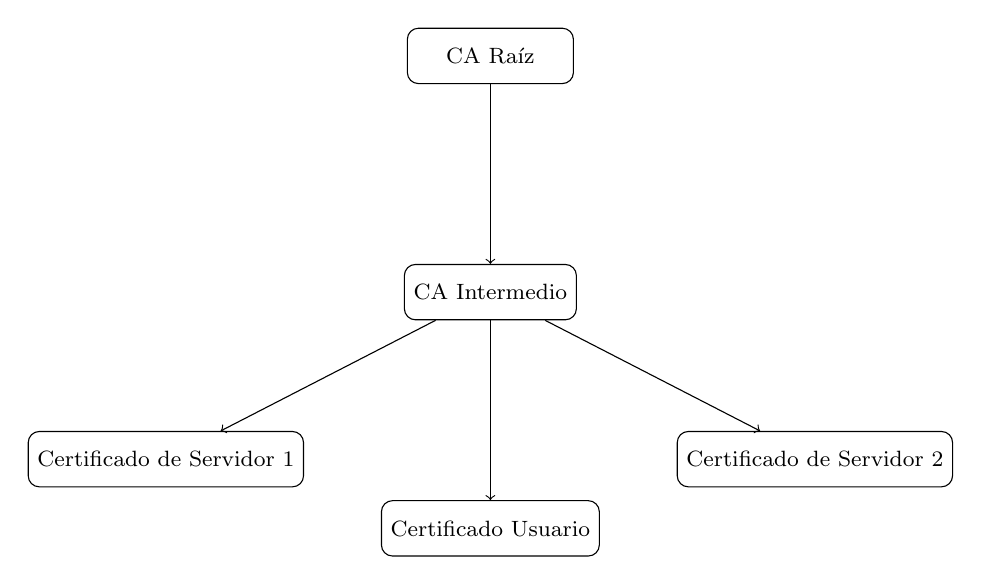
\begin{tikzpicture}[node distance=3cm, auto]

\tikzstyle{every node}=[font=\footnotesize]
\tikzstyle{ca} = [rectangle, draw, text centered, rounded corners, minimum height=2em, minimum width=6em]

% Nodos
\node[ca] (rootca) {CA Raíz};
\node[ca, below of=rootca] (intermediateca) {CA Intermedio};
\node[ca, below left of=intermediateca, xshift=-2cm] (servercert1) {Certificado de Servidor 1};
\node[ca, below right of=intermediateca, xshift=2cm] (servercert2) {Certificado de Servidor 2};
\node[ca, below of=intermediateca] (usercert) {Certificado Usuario};

% Lines
\draw[->] (rootca) -- (intermediateca);
\draw[->] (intermediateca) -- (servercert1);
\draw[->] (intermediateca) -- (servercert2);
\draw[->] (intermediateca) -- (usercert);

\end{tikzpicture}
\caption{Jerarquía de las Autoridades Certificadoras.}
\label{fig:ca-hierarchy}
\end{figure}

\subsection{Estándar de sintaxis de mensajes criptográficos (CMS)}

El Cryptographic Message Syntax (CMS), estandarizado en la RFC 5652, es un marco flexible para proteger mensajes. Este estándar define una sintaxis para encapsular datos firmados, cifrados, autenticados o comprimidos.

Una de las características más potentes de CMS es su capacidad para soportar arquitecturas de confianza jerárquicas mediante la inclusión de certificados. En un esquema de firma tradicional, el receptor necesita tener previamente la clave pública del remitente. CMS permite un modelo más dinámico:

\begin{enumerate}
    \item \textbf{Confianza anclada en la CA:} El verificador posee únicamente el certificado de una Autoridad de Certificación (CA) de confianza.

    \item \textbf{Estructura de datos firmados (SignedData):} El mensaje CMS encapsula no solo el contenido y la firma digital, sino también el certificado digital del firmante (y potencialmente toda la cadena de certificación hasta la CA raíz).

    \item \textbf{Proceso de validación:} Al recibir el mensaje, el verificador realiza una validación en dos etapas:
    \begin{itemize}
        \item Primero, extrae el certificado del firmante incluido en el mensaje y comprueba que es válido y que ha sido emitido por la CA de confianza que ya posee.
        \item Una vez validada la identidad del firmante, utiliza la clave pública contenida en ese certificado para verificar la firma digital del mensaje.
    \end{itemize}
\end{enumerate}

Este mecanismo desacopla la verificación de la identidad específica del firmante. Permite que el emisor rote sus claves o que existan múltiples entidades emisoras diferentes, siempre que todas posean certificados válidos emitidos por la CA común, el receptor podrá validar los mensajes sin necesidad de reconfiguración.

\section{Elección de algoritmos criptográficos}

Para este proyecto, la selección de algoritmos criptográficos se ha basado en las necesidades actuales del ecosistema IoT y en la gran diversidad de dispositivos que lo componen. El panorama IoT abarca desde dispositivos con recursos extremadamente limitados (pocos kilobytes de RAM y MHz de procesamiento) hasta dispositivos más potentes como gateways o sistemas embebidos basados en Linux. Esta heterogeneidad hace inviable la adopción de una única solución criptográfica que se adapte óptimamente a todos los escenarios.

Actualmente, el estándar de facto para el cifrado simétrico es AES (Advanced Encryption Standard). Este algoritmo es extremadamente robusto y eficiente en plataformas que disponen de recursos suficientes, especialmente aquellas que cuentan con aceleración por hardware (instrucciones AES-NI o similares). Sin embargo, en dispositivos restringidos sin soporte hardware específico, la implementación de AES puede resultar costosa en términos de ciclos de reloj, consumo de energía y uso de memoria, además de ser susceptible a ataques de canal lateral si no se implementa con complejas contramedidas.

En el ámbito de la criptografía asimétrica, y específicamente en lo referente a la firma digital, los estándares actuales más utilizados son RSA y ECDSA. Este último, basado en curvas elípticas, destaca por su eficiencia frente a RSA, permitiendo longitudes de clave mucho menores para un mismo nivel de seguridad. Adicionalmente, en este proyecto se tiene la intención de añadir soporte para ML-DSA (Module-Lattice-Based Digital Signature Standard), un algoritmo de firma post-cuántica que será detallado más adelante.

Por esta razón, se ha decidido ofrecer soporte para múltiples familias de algoritmos, permitiendo que cada despliegue seleccione la opción más adecuada según las capacidades del hardware objetivo.

\subsection{ASCON: Estándar de criptografía ligera}

ASCON ha sido seleccionado por el NIST (National Institute of Standards and Technology) como el estándar oficial de criptografía ligera para dispositivos con recursos limitados, publicado en la especificación NIST SP 800-232 \cite{NIST:SP800232:Ascon}. Esta selección consiste en un proceso de evaluación de varios años en el que ASCON demostró un equilibrio óptimo entre seguridad, eficiencia y versatilidad.

ASCON es una familia de algoritmos que proporciona:
\begin{itemize}
    \item \textbf{Cifrado autenticado (AEAD):} Garantiza confidencialidad e integridad en una sola operación.
    \item \textbf{Funciones hash:} Para verificación de integridad y generación de resúmenes criptográficos.
    \item \textbf{Autenticación de mensajes (MAC):} Para verificar la autenticidad sin cifrado.
\end{itemize}

Ascon cuenta con 3 variantes principales:

\begin{itemize}
    \item \textbf{Ascon-128:} La variante estándar que ofrece 128 bits de seguridad simétrica. Ideal para la mayoría de las aplicaciones IoT.
    \item \textbf{Ascon-128a:} Versión alternativa de alto rendimiento, que sacrifica ligeramente el tamaño del código por una mayor velocidad de procesamiento.
    \item \textbf{Ascon-80pq:} Variante de seguridad post-cuántica (post-quantum), diseñada con una clave de 160 bits para abordar desafíos de seguridad futuros.
\end{itemize}


\subsubsection{Ventajas de rendimiento frente a AES}

Según los benchmarks realizados por los autores de ASCON en el documento \textit{Status Update on Ascon v1.2} \cite{AsconStatusUpdate2022}, el algoritmo presenta ventajas significativas en dispositivos sin aceleración hardware para AES:

\begin{itemize}
    \item \textbf{Velocidad:} ASCON es entre 2 y 5 veces más rápido que AES-GCM en implementaciones software sobre microcontroladores de 8, 16 y 32 bits sin instrucciones AES dedicadas.
    \item \textbf{Tamaño de código:} La implementación de ASCON requiere significativamente menos memoria de programa que AES, lo cual es crítico en dispositivos con flash limitada.
    \item \textbf{Uso de RAM:} El estado interno de ASCON (320 bits) es compacto, reduciendo el consumo de memoria durante las operaciones criptográficas.
    \item \textbf{Tamaño de clave:} ASCON opera con claves de 128 bits, ofreciendo un nivel de seguridad adecuado teniendo en cuenta el objetivo de este, la criptografía ligera.
\end{itemize}

\subsubsection{Validación experimental}

Para validar la elección de ASCON, se decidió realizar pruebas experimentales en dos dispositivos representativos de entornos IoT con recursos limitados y sin aceleración por hardware para criptografía: una Raspberry Pi 3 \cite{RaspberryPi:Website} y un Arduino UNO R4 \cite{ArduinoIDE:Website}.

La implementación utilizada para las pruebas es la oficial de ASCON (versión 1.3.0) disponible en GitHub \cite{ASCON:Code:2023}, la cual es la recomendada por el NIST \cite{NIST:Website}.

Las pruebas en la Raspberry Pi 3 han consistido en el cifrado y descifrado de un fichero de 100 MB. Para asegurar la fiabilidad de los datos y reducir la variabilidad, se ejecutaron 100 iteraciones de cada prueba.

En el caso del Arduino, debido a las limitaciones inherentes de un microcontrolador, las pruebas fueron más restringidas. Se procedió probando con tamaños de texto plano (\textit{plaintext}) incrementales, desde pocos bytes hasta el límite permitido por la memoria del dispositivo.

Los resultados obtenidos para la Raspberry Pi 3 se muestran en la \autoref{fig:rpi_results}.

\begin{figure}[H]
    \centering
    \includegraphics[width=1\textwidth]{imagenes/desarrollo/rpi_results.png}
    \caption{Resultados de rendimiento en Raspberry Pi 3}
    \label{fig:rpi_results}
\end{figure}

Como se puede observar, ASCON confirma su superioridad frente a las variantes de AES, siendo entre 2 y 5 veces más rápido en este entorno sin aceleración hardware. Además, su rendimiento es equiparable al de ChaCha20-Poly1305, otro algoritmo conocido por su eficiencia en software.

Por otro lado, en el entorno más restringido del Arduino, los resultados son mucho más favorables para ASCON en todos los sentidos, como se aprecia en la \autoref{fig:arduino_results}.

\begin{figure}[H]
    \centering
    \includegraphics[width=0.8\textwidth]{imagenes/desarrollo/arduino_results.png}
    \caption{Resultados de rendimiento en Arduino UNO R4}
    \label{fig:arduino_results}
\end{figure}

ASCON resulta ser el claro ganador. Además, es importante destacar la eficiencia en el uso de memoria. En la \autoref{fig:max_plaintext_arduino} se muestra cómo ASCON permite cifrar y descifrar bloques de texto plano más grandes que el resto de algoritmos antes de agotar los recursos del microcontrolador, lo cual se atribuye a su menor consumo de memoria RAM.

\begin{figure}[H]
    \centering
    \includegraphics[width=0.8\textwidth]{imagenes/desarrollo/max_plaintext_arduino.png}
    \caption{Tamaño máximo de texto plano admitido en Arduino}
    \label{fig:max_plaintext_arduino}
\end{figure}

Adicionalmente, al considerar el uso de ASCON como algoritmo AEAD, el tamaño del tag de autenticación y los bytes adicionales que se añaden al texto plano son aspectos cruciales a evaluar. En la \autoref{fig:tag_tamaño} se ilustra la cantidad de bytes extra requeridos por cada algoritmo en comparación con el texto plano original. ASCON ocupa la mejor posición con solo 16 bytes adicionales, junto con AES-CTR y ChaCha20 sin autenticación.

\begin{figure}[H]
    \centering
    \includegraphics[width=0.8\textwidth]{imagenes/desarrollo/tag_tamaño.png}
    \caption{Bytes adicionales requeridos por algoritmos AEAD}
    \label{fig:tag_tamaño}
\end{figure}

\subsubsection{Consideraciones de seguridad post-cuántica}

Más allá de las ventajas de rendimiento, ASCON ofrece también protección contra amenazas futuras derivadas del desarrollo de computadores cuánticos. Según el NIST, algoritmos simétricos como AES-256 siguen siendo seguros a largo plazo incluso ante amenazas de computación cuántica \cite{NIST:SP800232:2023}. Esto se debe a que el algoritmo de Grover, que es el ataque cuántico más efectivo contra criptografía simétrica, reduce la seguridad efectiva a la mitad del tamaño de clave. Por ejemplo, una clave de 256 bits proporciona una seguridad equivalente a 128 bits ante un ataque cuántico, lo que sigue siendo considerado seguro por el NIST para aplicaciones sensibles.

Sin embargo, ASCON-80pq proporciona una protección algo más robusta. Esta variante está específicamente diseñada con una clave de 160 bits para garantizar 80 bits de seguridad efectiva incluso ante ataques cuánticos basados en el algoritmo de Grover \cite{NIST:SP800232:2023}. Si bien no es la variante más recomendada para entornos con recursos abundantes, donde AES-256 ofrecería una mayor seguridad a largo plazo, no está mal considerada, especialmente en dispositivos con recursos limitados o en entornos IoT donde la eficiencia computacional es un factor crítico. Esta característica lo hace particularmente atractivo para entornos IoT donde tanto la eficiencia computacional como la resistencia cuántica a largo plazo son requisitos críticos.

\subsubsection{Seguridad post cuantica en la firma digital: ML-DSA}

El panorama es significativamente diferente en el caso de la criptografía asimétrica. El algoritmo de Shor \cite{shor1997}, propuesto en 1997, demostró teóricamente que los sistemas criptográficos asimétricos actuales, como RSA y ECDSA, son completamente vulnerables a un computador cuántico suficientemente potente. Este algoritmo puede factorizar números grandes y resolver logaritmos discretos en tiempo polinómico, haciendo que los métodos de clave pública actuales sean obsoletos ante una amenaza cuántica.

En respuesta a esta amenaza, el NIST ha recomendado la transición hacia algoritmos basados en retículos (lattice-based cryptography). Para firmas digitales, el estándar recomendado es ML-DSA (Module-Lattice-Based Digital Signature Algorithm), estandarizado en el FIPS 204 \cite{NIST:FIPS204}. ML-DSA ofrece seguridad matemáticamente resistente a ataques cuánticos mientras mantiene una eficiencia computacional aceptable para la mayoría de aplicaciones, incluyendo dispositivos con recursos limitados.

Es importante destacar que, en términos de eficiencia de verificación, ML-DSA presenta un rendimiento competitivo frente a algoritmos tradicionales. Según benchmarks realizados en arquitecturas modernas x64 \cite{schemitt2025assessingimpactpostquantumdigital}, la verificación de una firma ML-DSA es más rápida que la de una curva elíptica equivalente (ECDSA), lo cual es relevante para dispositivos IoT que actúan frecuentemente como verificadores en procesos de actualización OTA. Por otro lado, la generación de firmas presenta tiempos similares e incluso mejores cuanto mayor sea el nivel de seguridad.

\begin{table}[H]
    \centering
    \small
    \begin{tabular}{|l|r|r|r|r|}
        \hline
        \textbf{Algoritmo} & \textbf{Firma (ms)} & \textbf{Verif. (ms)} & \textbf{Tam. clave (B)} & \textbf{Tam. firma (B)} \\
        \hline
        ECDSA P-521 (L5) & 0.1754 & 0.3126 & 66 & 132 \\
        ML-DSA-87 (L5) & 0.0956 & 0.0479 & 2592 & 4627 \\
        \hline
    \end{tabular}
    \caption{Comparativa de rendimiento y tamaños para nivel de seguridad 5 \cite{schemitt2025assessingimpactpostquantumdigital}}
    \label{tab:pq_benchmark_new}
\end{table}

Sin embargo, el punto crítico de ML-DSA radica en el tamaño de sus claves y firmas. A diferencia de ECDSA o RSA, ML-DSA requiere tamaños significativamente mayores. Por ejemplo, en el nivel de seguridad 5, mientras una firma ECDSA P-521 ocupa 132 bytes, una firma ML-DSA-87 asciende a 4627 bytes ($\sim$4.5 KB), lo que representa un incremento de aproximadamente 34 veces el tamaño (3405\% mayor). Este incremento impacta en el almacenamiento y el ancho de banda necesario para la transmisión de las firmas.

Si bien la transición no es urgente, dado que actualmente no existen computadores cuánticos capaces de ejecutar el algoritmo de Shor a escala práctica y todas las firmas verificadas hoy en día permanecen seguras, realizar el salto hacia algoritmos post-cuánticos es altamente recomendado para garantizar la seguridad a largo plazo.

La combinación de cifrado simétrico resistente a la computación cuántica (ASCON-80pq o AES-256-GCM) con firmas digitales basadas en retículos (ML-DSA) constituye un enfoque integral para garantizar la seguridad criptográfica a largo plazo, tanto ante amenazas actuales como futuras.

\section{Actualizaciones de software en sistemas embebidos}

La capacidad de actualizar el software de manera remota y segura (OTA - Over-The-Air) nos permiten, no solo corregir errores y vulnerabilidades de seguridad, sino también desplegar nuevas funcionalidades durante la vida útil del dispositivo.

Para comprender el diseño del sistema de actualizaciones propuesto, es necesario definir primero algunos conceptos clave del ecosistema Linux embebido.

\subsection{Conceptos fundamentales}

\subsubsection{Yocto Project}

El Proyecto Yocto es un proyecto de colaboración de código abierto que ayuda a los desarrolladores a crear sistemas personalizados basados en Linux para productos embebidos, independientemente de la arquitectura del hardware. Proporciona un conjunto flexible de herramientas y un espacio en el que los desarrolladores de sistemas embebidos de todo el mundo pueden compartir tecnologías, pilas de software, configuraciones y mejores prácticas que se pueden utilizar para crear imágenes de Linux personalizadas para dispositivos embebidos.

En la terminología de Yocto, se definen conceptos clave como \textit{recipes} (recetas), que son archivos que describen cómo obtener, configurar, compilar e instalar un paquete de software, y \textit{layers} (capas), que agrupan recetas relacionadas. Este sistema permite generar imágenes de sistema completas, incluyendo el bootloader, el kernel y el rootfs, de manera reproducible y controlada.

\subsubsection{Bootloader}

El \textit{bootloader} o gestor de arranque es el primer programa que se ejecuta cuando se enciende el dispositivo. Su responsabilidad principal es inicializar el hardware esencial (CPU, memoria RAM, relojes) y cargar el sistema operativo (kernel de Linux) en la memoria para su ejecución.

En el contexto de las actualizaciones OTA, el bootloader juega un papel crítico: es el componente encargado de decidir qué partición del sistema operativo se debe arrancar. Esto permite, por ejemplo, arrancar desde una nueva versión del software tras una actualización exitosa o volver a la versión anterior si la nueva falla. U-Boot (Universal Boot Loader) es el estándar de facto en sistemas Linux embebidos debido a su flexibilidad y soporte para múltiples arquitecturas.

\subsubsection{Rootfs (Sistema de archivos raíz)}

El \textit{rootfs} o sistema de archivos raíz es la estructura de directorios que contiene todos los archivos necesarios para que el sistema operativo funcione, incluyendo bibliotecas, binarios, archivos de configuración y las aplicaciones del usuario. En sistemas embebidos robustos, es común que el rootfs se monte en modo de solo lectura (\textit{read-only}) durante la operación normal. Esto protege la integridad del sistema frente a cortes de energía repentinos o corrupción de datos, asegurando que el dispositivo siempre arranque en un estado conocido.

\subsubsection{Estrategia de actualización A/B}

La estrategia de actualización A/B, también conocida como de doble partición o \textit{dual-copy}, es el mecanismo más robusto para garantizar actualizaciones seguras y atómicas. El almacenamiento del dispositivo se divide en dos conjuntos idénticos de particiones (Slot A y Slot B) para el sistema operativo (kernel y rootfs).

El funcionamiento es el siguiente:
\begin{itemize}
    \item El dispositivo arranca y opera desde una de las particiones (por ejemplo, Slot A), que se considera la partición "activa".
    \item Cuando se recibe una actualización, esta se instala en la partición inactiva (Slot B), sin interrumpir el funcionamiento del sistema.
    \item Una vez completada la instalación, se instruye al bootloader para que intente arrancar desde el Slot B en el próximo reinicio.
    \item Si el arranque del Slot B es exitoso, se marca como la nueva partición activa. Si falla (por ejemplo, el sistema se cuelga o no pasa los tests de arranque), el bootloader revierte automáticamente al Slot A, garantizando que el dispositivo siga operativo.
\end{itemize}

Este mecanismo proporciona redundancia y asegura que el dispositivo nunca quede inutilizado por una actualización fallida o corrupta, como se ilustra en la Figura~\ref{fig:ab_install}.

\begin{figure}[h]
\centering
\includegraphics[width=0.8\textwidth]{imagenes/desarrollo/AB_install.png}
\caption{Proceso de instalación de actualización A/B.}
\label{fig:ab_install}
\end{figure}

\subsection{SWUpdate: Gestor de actualizaciones}

SWUpdate es un framework de actualización de software de código abierto diseñado específicamente para sistemas Linux embebidos. A diferencia de gestores de paquetes tradicionales como \textit{apt} o \textit{dnf}, que actualizan archivos individuales, SWUpdate está orientado a la actualización de imágenes completas del sistema o particiones, lo cual es ideal para garantizar la consistencia en dispositivos IoT. Cabe destacar que SWUpdate es una de las soluciones recomendadas por el Proyecto Yocto para realizar actualizaciones de sistema completas y seguras \cite{Yocto:SystemUpdate}.

SWUpdate actúa como un agente que se ejecuta en el dispositivo y gestiona todo el proceso de actualización. Sus principales características y cualidades incluyen:

\begin{itemize}
    \item \textbf{Soporte para actualizaciones A/B:} Se integra nativamente con el bootloader (como U-Boot) para gestionar el cambio de particiones y el mecanismo de \textit{fallback} en caso de fallo.
    \item \textbf{Actualizaciones atómicas:} Garantiza que el sistema se actualice completamente o no se actualice en absoluto, evitando estados inconsistentes.
    \item \textbf{Streaming:} Permite instalar la actualización mientras se descarga, sin necesidad de almacenar el archivo completo en el almacenamiento local. Esto es crucial en dispositivos con memoria flash limitada.
    \item \textbf{Seguridad:} Soporta la verificación de imágenes firmadas digitalmente (utilizando RSA, CMS o claves simétricas) y el descifrado de imágenes, asegurando que solo software auténtico y autorizado pueda ser instalado.
    \item \textbf{Flexibilidad:} Es altamente configurable y soporta múltiples fuentes de actualización (USB, red, OTA) y formatos de imagen (raw, comprimidos con zstd/gzip, etc.).
\end{itemize}

En este proyecto, SWUpdate se utiliza como el componente central en el lado del dispositivo para orquestar la descarga, verificación e instalación de las nuevas versiones de firmware.

\subsubsection{Arquitectura modular}

Una de las características más destacadas de SWUpdate es su arquitectura altamente modular. El sistema dispone de gran cantidad de módulos o "handlers" que permiten gestionar diferentes tipos de artefactos (imágenes de disco, archivos, scripts, bootloaders) y comunicarse con diversos backends de gestión (SurBit, Hawkbit, servidores web genéricos, etc.).

En este proyecto en específico, se ha hecho uso del módulo \textbf{WFX} \cite{WFX}. Este módulo actúa como unión con el gestor de actualizaciones central c, encargándose de la comunicación con la plataforma de gestión en la nube donde WFX está ejecutado. A través del módulo WFX, el dispositivo puede consultar la disponibilidad de nuevas versiones, descargar los paquetes de actualización y reportar el estado final del proceso. El módulo WFX tiene soporte para dos tipos de actualizaciones: directo y por fases, donde el segundo requiere actividad del desarrollador. De todos modos, esto se detallará más en profundidad en la siguiente sección en conjunto con la herramienta WFX.

\subsubsection{Formato de paquete .swu y descriptor}

El paquete de actualización que maneja SWUpdate es un archivo con extensión \texttt{.swu}. Técnicamente, un archivo \texttt{.swu} es un contenedor en formato CPIO (\textit{Copy In, Copy Out}) que agrupa todos los elementos necesarios para la actualización. Dentro de este contenedor se encuentran:

\begin{itemize}
    \item \textbf{Imágenes de software:} Los binarios, sistemas de archivos o archivos individuales que se van a instalar (por ejemplo, imágenes \textit{raw} o archivos de firmware).
    \item \textbf{Scripts:} Scripts de pre-instalación o post-instalación si son necesarios.
    \item \textbf{Descriptor (sw-description):} El archivo más importante, que describe el contenido del paquete y las reglas de instalación.
\end{itemize}

El archivo \texttt{sw-description} utiliza una sintaxis basada en \textit{libconfig} y define metadatos como la versión, compatibilidad de hardware y la lista de archivos a instalar. A continuación se muestra un ejemplo de un descriptor básico:

\begin{verbatim}
software =
{
        version = "1.2";
        reboot = false;
        description = "Update vnull - OTA patch";
        hardware-compatibility: [ "1.0", "1.2", "1.3" ];

        ecs = {
                files: (
                        {
                                filename = "fichero";
                                path = "/ruta/fichero";
                                type = "rawfile";
                        }
                );
        }
}
\end{verbatim}

En este ejemplo, se define una actualización versión \enquote{1.2} compatible con varias revisiones de hardware. La sección \texttt{ecs} (que podría ser cualquier nombre de agrupación) contiene una lista de archivos, en este caso un único archivo de tipo \texttt{rawfile} que se copiará a la ruta especificada.

\subsubsection{Flujo de actualización (Pulling)}

El proceso de actualización en este proyecto sigue un modelo de "pulling" (sondeo), donde la iniciativa parte del dispositivo. El funcionamiento típico con el gestor de actualizaciones es el siguiente:

\begin{enumerate}
    \item \textbf{Comprobación (Polling):} El servicio SWUpdate en el dispositivo consulta periódicamente al servidor central (a través del módulo WFX) si existe una nueva actualización disponible para su versión de hardware y software actual.
    \item \textbf{Descarga:} Si el servidor responde afirmativamente con una actualización pendiente, el dispositivo comienza la descarga del archivo \texttt{.swu}.
    \item \textbf{Instalación:} SWUpdate procesa el archivo \texttt{.swu}, lee el descriptor \texttt{sw-description} y procede a instalar los artefactos según las reglas definidas.
    \item \textbf{Confirmación:} Una vez finalizada la instalación, el dispositivo reporta el éxito o fracaso de la operación al servidor.
\end{enumerate}

\subsection{Generación de paquetes: SWUGenerator}

Para la creación de los paquetes de actualización \texttt{.swu}, existe una herramienta complementaria denominada \textbf{SWUGenerator} \cite{SWUGenerator}. Esta utilidad, escrita en Python y desarrollada por los mismos creadores de SWUpdate (Stefano Babic), simplifica significativamente el proceso de empaquetado.

SWUGenerator toma como entrada los archivos que componen la actualización (imágenes de sistema, scripts, etc.) y un archivo de configuración simplificado, y se encarga de construir automáticamente el contenedor CPIO dado el descriptor y ficheros.

Una de las características más potentes de SWUGenerator es su capacidad para integrar la seguridad en el proceso de construcción. Permite, mediante parámetros de línea de comandos o configuración, firmar digitalmente el paquete utilizando los mismos algoritmos criptográficos soportados por SWUpdate (RSA, CMS, etc.). Asimismo, cabe destacar que los mecanismos de cifrado y firma son los mismos que los utilizados en SWUpdate, garantizando la compatibilidad total entre la generación y la instalación de los paquetes. Esto supone que, de añadir nuevos algoritmos en SWUpdate, SWUGenerator también necesitaría ser actualizado para soportarlos.

\subsection{WFX: Workflow Executioner}

WFX (\textit{Workflow Executioner}) es una herramienta desarrollada por Siemens y escrita en el lenguaje de programación Go, diseñada para gestionar la ejecución de flujos de trabajo (\textit{workflows}) en entornos distribuidos. En el contexto de este proyecto, WFX actúa como el gestor del sistema de actualizaciones OTA, orquestando el ciclo de vida de las actualizaciones desde que se definen hasta que se instalan en los dispositivos.

El funcionamiento de WFX se basa en máquinas de estados cliente-servidor. Un flujo de trabajo define una serie de estados por los que debe pasar una tarea (en este caso, una actualización) y las transiciones permitidas entre ellos. Estas transiciones pueden ser desencadenadas por el dispositivo (el cliente, a través de SWUpdate) o por el operador del sistema (el desarrollador o administrador).

Para facilitar esta interacción, WFX expone dos APIs diferenciadas:
\begin{itemize}
    \item \textbf{API Norte (North API):} Destinada al desarrollador o a los sistemas de gestión. Permite crear trabajos, monitorizar su estado y ejecutar transiciones administrativas (como aprobar una actualización).
    \item \textbf{API Sur (South API):} Destinada a los dispositivos. Es utilizada por el agente SWUpdate (a través del módulo WFX) para consultar tareas pendientes, reportar progreso y actualizar el estado de la instalación.
\end{itemize}

\subsubsection{Tipos de Workflows}

WFX integra flujos de trabajo específicos para la actualización de artefactos en dispositivos, conocidos como DAU (\textit{Device Artifact Update}). El sistema soporta dos modalidades principales: \textit{Direct} (Directo) y \textit{Phased} (Por fases).


El \textbf{Workflow Directo} es un proceso automatizado diseñado para despliegues rápidos donde no se requiere intervención manual. Una vez creado el trabajo, el dispositivo procede a la descarga e instalación sin pausas intermedias, como se muestra en la Figura \ref{fig:workflow_direct}.

\begin{figure}[h]
    \centering
    \includegraphics[width=0.4\textwidth]{imagenes/desarrollo/direct.png}
    \caption{Diagrama de estados del Workflow Directo.}
    \label{fig:workflow_direct}
\end{figure}


El \textbf{Workflow Por Fases} introduce puntos de control manual para una gestión más controlada del despliegue. Es fundamental notar los estados marcados con los símbolos \texttt{<>} en el diagrama de la Figura \ref{fig:workflow_phased}. Estos estados indican que la transición no es automática, sino que requiere una acción explícita por parte del desarrollador a través de la API Norte. Específicamente, estas intervenciones son necesarias para dar inicio a la actualización y para activarla una vez instalada, permitiendo un control granular sobre el despliegue.

\begin{figure}[H]
    \centering
    \includegraphics[width=0.4\textwidth]{imagenes/desarrollo/phased.png}
    \caption{Diagrama de estados del Workflow Por Fases.}
    \label{fig:workflow_phased}
\end{figure}


Además de los flujos de trabajo predefinidos, WFX permite la creación de \textbf{Workflows personalizados}. Estos flujos pueden adaptarse a necesidades específicas del proyecto, incorporando estados adicionales, transiciones únicas o integraciones con otros sistemas. La flexibilidad para definir workflows personalizados es una característica poderosa que permite a los desarrolladores diseñar procesos de actualización que se alineen perfectamente con los requisitos operativos y de seguridad de su entorno. Sin embargo, esto supone un esfuerzo adicional también en la implementación del lado del dispositivo, ya que el agente SWUpdate debe ser capaz de manejar los nuevos estados y transiciones definidos.

\subsubsection{La Entidad Job}

En la arquitectura de WFX, cuando se asigna una actualización a un dispositivo, se crea una entidad denominada \textbf{Job} (Trabajo). El agente SWUpdate en el dispositivo sondea constantemente la API Sur de WFX buscando si existe algún \textit{Job} activo asignado a su \textit{DeviceID}.

Un \textit{Job} encapsula toda la información necesaria para realizar la actualización, tal y como se ilustra en la Figura \ref{fig:job_definition}. Sus componentes principales son:

\begin{figure}[h]
    \centering
    \includegraphics[width=0.6\textwidth]{imagenes/desarrollo/job_definition.png}
    \caption{Estructura de la entidad Job en WFX.}
    \label{fig:job_definition}
\end{figure}

\begin{itemize}
    \item \textbf{ID:} Identificador único del trabajo.
    \item \textbf{DeviceID:} Identificador del dispositivo al que está asignado el trabajo.
    \item \textbf{Workflow:} Nombre del flujo de trabajo que rige este trabajo (ej. \texttt{wfx.workflow.dau.direct}).
    \item \textbf{Tags:} Etiquetas para categorización y búsquedas.
    \item \textbf{State:} Estado actual del trabajo dentro del flujo (ej. \texttt{CREATED}, \texttt{DOWNLOADING}, \texttt{INSTALLED}).
    \item \textbf{Progress:} Indicador numérico del progreso de la tarea.
    \item \textbf{Message:} Mensajes de log o errores reportados por el dispositivo.
    \item \textbf{Hash:} Valor hash para identificar y verificar la integridad del trabajo.
    \item \textbf{Fechas:} \textit{Start time} (inicio) y \textit{Modification time} (última actualización).
    \item \textbf{History:} Un registro histórico en formato JSON que almacena la evolución del trabajo, incluyendo cambios de estado, tiempos de modificación y mensajes.
\end{itemize}

Un componente crítico del \textit{Job} es el campo \textbf{Definition} (metadatos). Este campo se almacena como un objeto JSON y contiene los detalles técnicos de la actualización que el dispositivo necesita procesar. En este proyecto, el campo \textit{Definition} se ha utilizado para inyectar identificadores y configuraciones específicas:

\begin{itemize}
    \item \textbf{Artifacts:} Lista de objetos a instalar. Cada artefacto incluye un \textbf{Name} y una \textbf{Uri} (ruta de descarga para el dispositivo).
    \item \textbf{Version:} Versión del paquete de software.
    \item \textbf{Type:} Tipo de actualización.
    \item \textbf{Campos personalizables:} Se pueden incluir campos adicionales según las necesidades del proyecto, como por ejemplo, el identificador de la campaña de actualización, el tipo de dispositivo o cualquier otro dato relevante para la lógica de negocio del sistema de actualizaciones.
\end{itemize}

\subsection{LamassuIoT}

Lamassu es una infraestructura de clave pública (PKI) diseñada específicamente para dispositivos IoT. Ofrece capacidades completas para la gestión de claves asimétricas, autoridades certificadoras (CA) y certificados digitales. Esta infraestructura se integra directamente con los dispositivos, permitiéndoles utilizar estos materiales criptográficos para procesos de autenticación robusta.

Un concepto central en Lamassu es el DMS (\textit{Device Management System}). Un DMS actúa como una agrupación lógica de dispositivos, permitiendo administrar flotas de dispositivos de manera organizada. En el contexto de una arquitectura IoT, un DMS puede representar una zona geográfica, un tipo de dispositivo específico o un cliente particular.

En el alcance de este proyecto, Lamassu desempeña un papel fundamental como proveedor de identidad y seguridad:
\begin{itemize}
    \item \textbf{Gestión de Dispositivos:} Provee las listas de dispositivos autorizados y sus agrupaciones (DMS).
    \item \textbf{Infraestructura de Confianza:} Suministra los mecanismos de firma digital y emisión de certificados necesarios para validar la autenticidad del firmware y de los propios dispositivos.
\end{itemize}

\subsection{Extensión del KMS para Criptografía Simétrica}

Es importante destacar que, en su estado actual, Lamassu no disponía de un sistema de gestión de claves (KMS) para criptografía simétrica. Como parte de los objetivos de este trabajo, se ha desarrollado esta capacidad, extendiendo el KMS de Lamassu para soportar:

\begin{itemize}
    \item \textbf{Gestión de claves simétricas:} Generación, importación, almacenamiento y rotación de claves para algoritmos de cifrado simétrico (AES en sus variantes y ASCON).
    \item \textbf{Operaciones de cifrado/descifrado:} Ejecución de operaciones criptográficas directamente en el KMS, manteniendo las claves protegidas sin exponerlas.
    \item \textbf{Generación de MAC (Message Authentication Code):} Soporte para algoritmos de autenticación de mensajes, incluyendo AES-CMAC y ASCON-MAC, permitiendo verificar la integridad y autenticidad de los datos sin cifrarlos.
\end{itemize}

Esta extensión permite que el servicio de Updates utilice el KMS de Lamassu para todas las operaciones criptográficas necesarias en el proceso de creación de paquetes de actualización, garantizando una gestión centralizada y segura de las claves criptográficas.

\section{Infraestructura Planteada}

La arquitectura propuesta para la plataforma de actualizaciones seguras se ha diseñado con el objetivo de desacoplar la complejidad de la gestión de actualizaciones de la lógica de negocio, proporcionando una interfaz unificada y segura para los desarrolladores.

Como se ha mencionado anteriormente, \textbf{WFX} actúa como el motor de distribución de las actualizaciones. Es el componente encargado de mantener el estado de los despliegues y servir las actualizaciones a los dispositivos. En el lado del dispositivo, la herramienta \textbf{SWUpdate} es la responsable de realizar el \textit{polling} periódico hacia WFX para comprobar si existen nuevas tareas asignadas, y en caso afirmativo, descargar e instalar la actualización siguiendo el flujo definido.

Para orquestar todo este proceso y facilitar su gestión, se introduce un nuevo servicio denominado \textbf{Updates}. Este módulo actúa como una capa de abstracción y control sobre WFX. Sus responsabilidades principales incluyen:

\begin{itemize}
    \item \textbf{Construcción de Paquetes:} Utilizar la herramienta \textbf{SWUGenerator} para crear los paquetes de actualización a partir de los ficheros proporcionados por el desarrollador, generando el formato SWU requerido por SWUpdate.
    \item \textbf{Gestión de Versiones:} Administrar el catálogo de versiones de software disponibles.
    \item \textbf{Gestión de Despliegues:} Coordinar la creación y supervisión de las campañas de actualización.
    \item \textbf{Interacción con WFX:} Comunicarse con la API de WFX para crear los trabajos (\textit{Jobs}) y monitorizar su progreso, ocultando esta complejidad al usuario final.
    \item \textbf{Integración con Lamassu:} Utilizar los servicios de \textbf{KMS} (Key Management System) para las operaciones criptográficas (cifrado y firma de paquetes) y el servicio \textbf{DMS} (Device Management System) para obtener la información de los dispositivos y sus agrupaciones.
\end{itemize}

De esta manera, el desarrollador puede desplegar actualizaciones utilizando este servicio sin necesidad de interactuar directamente con los detalles de bajo nivel de WFX o la gestión de claves.

Adicionalmente, se ha desarrollado una \textbf{Interfaz Web} que proporciona una experiencia de usuario visual para la gestión del sistema. Esta interfaz se comunica con la API REST expuesta por el servicio de Updates, permitiendo a los administradores subir nuevos firmwares, definir estrategias de actualización y visualizar el estado de la flota de dispositivos en tiempo real.

La arquitectura global de la solución y la interacción entre estos componentes se ilustra en la \autoref{fig:plataforma_arquitectura}.

\begin{figure}[H]
    \centering
    \includegraphics[width=1\textwidth]{imagenes/desarrollo/plataforma.png}
    \caption{Arquitectura de la plataforma de actualizaciones propuesta}
    \label{fig:plataforma_arquitectura}
\end{figure}

\section{Casos de Uso del Sistema}

Una vez presentada la arquitectura de la plataforma, resulta fundamental identificar y describir los principales casos de uso que ilustran las interacciones entre los diferentes actores y componentes del sistema. Esta sección define quiénes interactúan con la plataforma y cómo lo hacen, proporcionando una visión funcional del sistema antes de profundizar en los detalles técnicos de implementación.

\subsection{Actores del sistema}

Los actores principales que interactúan con la plataforma son:

\begin{itemize}
    \item \textbf{Desarrollador:} Usuario responsable de gestionar las actualizaciones, crear paquetes de actualización, configurar campañas de despliegue y monitorizar el estado de la flota de dispositivos. Interactúa con el sistema a través de la interfaz web y, ocasionalmente, mediante la API REST del servicio Updates.

    \item \textbf{Dispositivo IoT:} Dispositivo embebido que ejecuta el agente SWUpdate y realiza consultas periódicas (polling) al sistema WFX para comprobar la disponibilidad de nuevas actualizaciones, descargarlas e instalarlas.
\end{itemize}

\subsection{Componentes del sistema}

La plataforma OTA se organiza en dos subsistemas principales:

\begin{itemize}
    \item \textbf{Backend:} Módulo de gestión centralizada (Updates) que proporciona las funcionalidades de creación, versionado, cifrado y firma de paquetes de actualización. Se integra con Lamassu para las operaciones criptográficas.

    \item \textbf{WFX:} Motor de orquestación de workflows que mantiene el estado de las tareas de actualización y actúa como punto de sincronización entre el backend y los dispositivos.
\end{itemize}

Como se ha comentado anteiormente, el sistema se integra con:

\begin{itemize}
    \item \textbf{Lamassu PKI:} Infraestructura de gestión de identidades, claves y certificados que proporciona los servicios criptográficos necesarios para firma y cifrado de paquetes, así como la gestión de dispositivos (DMS) y sus agrupaciones.
\end{itemize}

\subsection{Diagrama de casos de uso}

La \autoref{fig:use_cases} presenta el diagrama de casos de uso del sistema, mostrando las principales interacciones entre los actores y los subsistemas de la plataforma.

\begin{figure}[H]
    \centering
    \includegraphics[width=0.9\textwidth]{imagenes/desarrollo/casosusootaq.png}
    \caption{Diagrama de casos de uso de la plataforma de actualizaciones OTA}
    \label{fig:use_cases}
\end{figure}

\subsection{Descripción de los casos de uso}

El sistema se organiza en dos subsistemas principales dentro de la Plataforma OTA, cada uno con sus casos de uso específicos:

\subsubsection{Casos de uso del Backend}

Los casos de uso gestionados por el desarrollador en el subsistema Backend son:

\begin{itemize}
    \item \textbf{Crear actualización:} El desarrollador proporciona los archivos de firmware o software que componen la nueva versión. El sistema valida los archivos y los prepara para su empaquetado.

    \item \textbf{Gestionar versión:} El desarrollador define los metadatos de la versión (nombre, número de versión, si es firmware...).

    \item \textbf{Firmar/Encriptar actualización (<<include>> desde Lamassu):} Tanto la creación como la gestión de versiones permiten operaciones criptográficas. El desarrollador selecciona las claves de cifrado simétricas y las claves privadas para firma digital desde Lamassu. El sistema utiliza el KMS de Lamassu para cifrar el paquete (con algoritmos como AES-256-GCM o ASCON-128a) y firmar digitalmente el contenido (con RSA, ECDSA o ML-DSA post-cuántico), generando un paquete .swu firmado y cifrado.

    \item \textbf{Lanzar actualización:} El desarrollador configura una campaña de despliegue, especificando la estrategia de despliegue (por porcentajes o cantidades fijas de dispositivos), el tipo de workflow (directo o por fases) y el modo de progresión (automático o manual).

    \item \textbf{Crear tarea (<<include>> en WFX):} Al lanzar una actualización, el backend crea automáticamente tareas (Jobs) en WFX para cada dispositivo o batch de dispositivos objetivo, inyectando los metadatos necesarios (URI del paquete, algoritmos de cifrado/firma, identificadores).

    \item \textbf{Ver estado lanzamiento:} El desarrollador monitoriza el progreso de la campaña de actualización a través de la interfaz web, visualizando cuántos dispositivos han completado exitosamente, cuántos están en progreso y cuántos han fallado.

    \item \textbf{Consultar tarea (<<include>> en WFX):} Para obtener el estado actualizado del lanzamiento, el backend consulta el estado de los Jobs en WFX, agregando la información de todos los dispositivos para presentarla al desarrollador.
\end{itemize}

\subsubsection{Casos de uso de WFX}

Los casos de uso gestionados por el dispositivo IoT en el subsistema WFX son:

\begin{itemize}
    \item \textbf{Consultar tarea:} El dispositivo realiza polling periódico a la API Sur de WFX consultando si existe algún Job (tarea de actualización) asignado a su DeviceID. Si existe una tarea pendiente, descarga los metadatos del Job, incluyendo la URI del paquete, el algoritmo de cifrado y firma utilizado, y el tipo de workflow a seguir.

    \item \textbf{Descargar actualización:} Una vez detectada una tarea pendiente, el dispositivo descarga el paquete .swu detallado en el Job. Durante el proceso, verifica la firma digital del paquete contra el certificado de la CA raíz configurada localmente, confirma la integridad criptográfica, descifra el contenido utilizando la clave simétrica correspondiente al algoritmo especificado (almacenada previamente en el dispositivo) y procede con la instalación. Finalmente, actualiza el estado del Job en WFX, reportando el progreso y resultado de la operación (éxito o fallo).
\end{itemize}

\subsection{Diagramas de Secuencia}

Los diagramas de secuencia siguientes detallan la comunicación entre los distintos servicios de la plataforma para cada uno de los flujos principales del sistema.

\subsubsection{Creación de un Update Pack}

El diagrama de la \autoref{fig:seq_updatepack} ilustra el flujo de creación de un paquete de actualización. El punto más destacable es la integración con Lamassu para las operaciones criptográficas: en lugar de gestionar las claves localmente, el servicio Updates delega la firma del paquete en el KMS de Lamassu a través de SWUGenerator. De este modo, la clave privada nunca abandona la infraestructura PKI y el paquete resultante incorpora el certificado en la estructura CMS para su posterior verificación en el dispositivo.

\begin{figure}[H]
    \centering
    \includegraphics[width=1\textwidth]{imagenes/desarrollo/DiagramasSecuencia-UpdateUPDPack.png}
    \caption{Diagrama de secuencia de creación de un Update Pack}
    \label{fig:seq_updatepack}
\end{figure}

\subsubsection{Lanzamiento de una Actualización}

La \autoref{fig:seq_lanzamiento} muestra el flujo de lanzamiento de una campaña de actualización. Se aprecian dos interacciones clave con la infraestructura Lamassu: primero, la consulta al \textit{Device Manager} (DMS) para obtener la lista de dispositivos asociados al grupo objetivo; segundo, la creación de un \textit{Job} en WFX por cada dispositivo, inyectando los metadatos necesarios (URI del paquete, algoritmo de cifrado y firma) para que cada agente SWUpdate pueda procesarlo de forma autónoma.

\begin{figure}[H]
    \centering
    \includegraphics[width=1\textwidth]{imagenes/desarrollo/DiagramasSecuencia-Lanzamiento de Actualización.png}
    \caption{Diagrama de secuencia de lanzamiento de una actualización}
    \label{fig:seq_lanzamiento}
\end{figure}

\subsubsection{Flujo en el Dispositivo}

El diagrama de la \autoref{fig:seq_device} describe el comportamiento del agente SWUpdate en el dispositivo. El flujo se basa en un modelo de \textit{polling}: el dispositivo consulta periódicamente la API Sur de WFX buscando tareas asignadas a su \textit{DeviceID}. Cuando detecta un Job activo, descarga el paquete desde la URI indicada en los metadatos, verifica la firma y descifra el contenido, instala la actualización en la partición inactiva y finalmente reporta el resultado a WFX para cerrar el ciclo.

\begin{figure}[H]
    \centering
    \includegraphics[width=1\textwidth]{imagenes/desarrollo/DiagramasSecuencia-device.png}
    \caption{Diagrama de secuencia del flujo de actualización en el dispositivo}
    \label{fig:seq_device}
\end{figure}

\section{Modelo de Datos}

Para entender el módulo de Updates y su integración con Lamassu y WFX, es fundamental definir las entidades principales que componen el modelo de datos del sistema. Estas entidades representan los conceptos clave y las estructuras de información que se manejan en la plataforma de actualizaciones.

\subsection{Entidades de Lamassu IoT}

Desde la infraestructura Lamassu se obtienen dos entidades fundamentales que proporcionan la base organizativa y de identidad del sistema:

\begin{itemize}
    \item \textbf{Device (Dispositivo):} Representa cada dispositivo IoT registrado en el sistema. Cada dispositivo contiene información de identificación, credenciales y metadatos asociados a su configuración de seguridad.

    \item \textbf{DMS (Device Management System):} Agrupa lógicamente conjuntos de dispositivos. Un DMS puede representar una flota de dispositivos de un cliente específico, una zona geográfica determinada, o cualquier otra agrupación organizativa. Esta entidad es clave para aplicar políticas de actualización a grupos completos de dispositivos.
\end{itemize}

\subsection{Entidades de WFX}

El sistema de orquestación de flujos de trabajo WFX aporta las siguientes entidades:

\begin{itemize}
    \item \textbf{Workflow:} Define el flujo de estados por los que pasa una actualización. Como se ha descrito anteriormente, existen workflows predefinidos como \textit{Direct} y \textit{Phased}, y es posible crear workflows personalizados adaptados a necesidades específicas.

    \item \textbf{Job:} Representa una instancia de actualización asignada a un dispositivo concreto. Encapsula toda la información necesaria para llevar a cabo la actualización, incluyendo el estado actual, progreso, historial de cambios, y los metadatos técnicos de la actualización en su campo \textit{Definition}.
\end{itemize}

\subsection{Entidades del Módulo Updates}

El módulo de Updates introduce dos entidades primordiales que gestionan el ciclo de vida de las actualizaciones:

\subsubsection{Update-Pack (Paquete de Actualización)}

El \textbf{Update-Pack} es la entidad que representa una actualización disponible en el sistema. Contiene toda la información necesaria para construir, cifrar y firmar el paquete de actualización. Sus campos principales son:

\begin{itemize}
    \item \textbf{Name:} Nombre identificativo del paquete de actualización.
    \item \textbf{Version:} Versión del software o firmware contenido en el paquete.
    \item \textbf{Type:} Tipo de actualización, que puede ser \textit{firmware} (actualización completa del sistema embebido) o \textit{file} (fichero específico o componente de software).
    \item \textbf{Alg\_Enc:} Algoritmo de cifrado utilizado para proteger el contenido del paquete (ej. AES-256, ASCON).
    \item \textbf{Alg\_Sign:} Algoritmo de firma digital utilizado para garantizar la autenticidad e integridad del paquete (ej. RSA, ECDSA).
    \item \textbf{IV (Initialization Vector):} Vector de inicialización utilizado en el proceso de cifrado simétrico.
    \item \textbf{Descriptor\_Encrypted:} Indicador booleano que especifica si el descriptor del paquete está cifrado .
\end{itemize}

Esta entidad permite mantener un catálogo versionado de actualizaciones, facilitando el control de versiones y la trazabilidad de cada paquete desplegado.

\subsubsection{Launch (Lanzamiento)}

El \textbf{Launch} representa una campaña de despliegue de una versión específica de actualización. A diferencia del Update-Pack que define \textit{qué} se actualiza, el Launch define \textit{cómo} y \textit{cuándo} se despliega. Sus campos principales son:

\begin{itemize}
    \item \textbf{ID:} Identificador único del lanzamiento.
    \item \textbf{ExecDate:} Fecha y hora de ejecución programada del lanzamiento.
    \item \textbf{Workflow\_Type:} Tipo de workflow utilizado para este lanzamiento (ej. \textit{Direct}, \textit{Phased}, o un workflow personalizado).
    \item \textbf{Devices\_Completed:} Número de dispositivos que han completado exitosamente la actualización.
    \item \textbf{Devices\_Not\_Started:} Número de dispositivos que aún no han iniciado el proceso de actualización.
    \item \textbf{Active\_Devices:} Número de dispositivos que están actualmente ejecutando la actualización.
    \item \textbf{Rollout:} Estrategia de despliegue, que puede ser por porcentaje (\textit{\%}) o cantidad fija (\textit{fixed}).
    \item \textbf{Rollout\_Value:} Valor asociado a la estrategia de rollout (porcentaje o número de dispositivos).
    \item \textbf{Rollout\_Mode:} Modo de progresión entre batches, que puede ser \textit{auto} (automático) o \textit{manual}.
    \item \textbf{Test\_Device\_ID:} Identificador del dispositivo utilizado para pruebas piloto antes del despliegue.
    \item \textbf{Launched\_Version:} Referencia a la versión del Update-Pack que se está desplegando.
\end{itemize}

El Launch permite implementar estrategias de despliegue gradual (\textit{phased rollout}), minimizando riesgos al actualizar primero un subconjunto de dispositivos antes de extender la actualización a toda la flota.

Las actualizaciones se despliegan organizadas en batches (lotes) de dispositivos según la estrategia definida en el campo \textit{Rollout}. El sistema ofrece dos modos de progresión entre batches:

\begin{itemize}
    \item \textbf{Modo Automático:} Una vez que todos los dispositivos de un batch completan exitosamente la actualización, el sistema procede automáticamente a lanzar el siguiente batch sin intervención manual. Este modo es ideal para despliegues donde se confía en la estabilidad de la actualización y se desea una distribución rápida.

    \item \textbf{Modo Manual:} Tras la finalización de cada batch, el sistema espera confirmación explícita del desarrollador o administrador antes de proceder con el siguiente lote. Este enfoque proporciona un mayor control y permite verificar el comportamiento de la actualización en producción antes de expandir el despliegue, siendo especialmente útil para actualizaciones críticas o de alto riesgo.
\end{itemize}

\subsection{Relaciones entre Entidades}

Las relaciones entre las entidades del sistema se establecen de la siguiente manera:

\begin{itemize}
    \item Un \textbf{DMS} puede tener asociados múltiples \textbf{Update-Packs}, permitiendo gestionar diferentes versiones de software para una misma agrupación de dispositivos.

    \item Un \textbf{DMS} puede tener múltiples \textbf{Launches}, posibilitando campañas de actualización sucesivas o paralelas para diferentes componentes.

    \item Un \textbf{Launch} está asociado a un único \textbf{Update-Pack}, estableciendo una relación unívoca entre cada campaña de despliegue y la versión de software que distribuye.

    \item Cada \textbf{Job} creado en WFX está vinculado a un único dispositivo que forme parte del lanzamiento, por lo que en un lanzamiento finalizado habra tantos jobs como dispositivos planeados a actualizar.
\end{itemize}

La \autoref{fig:data_model} ilustra el diagrama completo del modelo de datos, mostrando cómo se relacionan las entidades del módulo de Updates con las entidades de Lamassu y WFX.

\begin{figure}[H]
    \centering
    \includegraphics[width=0.9\textwidth]{imagenes/desarrollo/data_model.png}
    \caption{Diagrama del modelo de datos de la plataforma}
    \label{fig:data_model}
\end{figure}

\section{Integración de Criptografía Ligera y Post-Cuántica}

Una de las contribuciones principales de este trabajo es la integración de algoritmos criptográficos ligeros (LWC) y resistentes a ataques cuánticos (PQ) en la cadena de actualización de dispositivos IoT. Esta integración ha requerido modificaciones tanto en SWUpdate como en SWUGenerator, presentando desafíos técnicos considerables.

\subsection{Integración de Algoritmos de Cifrado Simétrico}

La incorporación de nuevas alternativas de criptografía simétrica, en particular ASCON, si bien swupdate es muy personalizable, este cambio ha supuesto una dificultad considerable. Originalmente, SWUpdate únicamente admitía cifrado simétrico mediante AES-CBC, sin ningún mecanismo de selección de algoritmo. Esta restricción se debía a que, al existir una sola opción, no se requería un selector explícito en el diseño original.

Para superar esta limitación, se ha modificado el código fuente de SWUpdate para incorporar las siguientes capacidades:

\begin{itemize}
    \item \textbf{Selector de algoritmo:} Posibilidad de definir explícitamente qué algoritmo de cifrado se utilizará.
    \item \textbf{Soporte para variantes de AES:} Integración de las variantes CBC, CTR y GCM de AES para las longitudes de clave de 128, 192 y 256 bits.
    \item \textbf{Soporte para ASCON:} Integración de la implementación en C de ASCON en su variante más eficiente.
\end{itemize}

Por defecto, el sistema asume que las claves criptográficas se encuentran almacenadas en la ruta \texttt{/etc/swupdate/}\texttt{keys/alg\_variant.key}, siguiendo una convención de nomenclatura que incluye el algoritmo con sub variante, el IV y la clave.

\subsubsection{Instalación Nativa}

Para mantener la flexibilidad y no cerrar puertas a diferentes escenarios de uso, se ha conservado la opción de instalación nativa. Esto puede ocurrir si se requiere de una instalación mediante USB practica muy común en el ambito de dispositivos linux embebidos. En este modo, el algoritmo y la clave se especifican directamente por línea de comandos:

\begin{verbatim}
swupdate -i test.swu -K ./test\_key.key
\end{verbatim}


\subsubsection{Integración con WFX}

En el caso de despliegues orquestados mediante WFX, la información del algoritmo de cifrado se transmite a través de los metadatos del Job. Al recibir una tarea pendiente, el agente SWUpdate extrae el algoritmo especificado en el campo \textit{definition}, que WFX proporciona para usos personalizados.

El formato de metadatos utilizado en los Jobs de WFX es el siguiente:

\begin{lstlisting}[caption={Formato de metadatos del Job en WFX}, label={lst:wfx_metadata}]
{
  "id": "update-001",
  "definition": {
    "artifacts": [
      {
        "uri": "https://cdn.example.com/firmware.swu.enc",
        "ivt": "0123456789abcdef0123456789abcdef",
        "algorithm": "aes256-cbc"
      }
    ]
  }
}
\end{lstlisting}

Los campos clave son:
\begin{itemize}
    \item \textbf{uri:} Ubicación desde donde el dispositivo descargará el paquete de actualización.
    \item \textbf{ivt:} Vector de inicialización utilizado en el cifrado.
    \item \textbf{algorithm:} Algoritmo de cifrado empleado (ej. \texttt{aes256-cbc}, \texttt{ascon-128a}).
\end{itemize}

\subsection{Integración de Firma Digital Post-Cuántica}

La integración de mecanismos de firma digital resistentes a ataques cuánticos resultó relativamente más sencilla que la del cifrado simétrico. El proceso requirió dos modificaciones principales:

\begin{enumerate}
    \item \textbf{Habilitación en menuconfig:} SWUpdate utiliza un sistema de configuración basado en Kconfig (similar al kernel de Linux) que permite habilitar o deshabilitar características antes de compilar (\textit{buildear}) el proyecto. Se habilitaron los métodos de firma en esta configuración, en especifico verificación de firma con formato CMS.

    \item \textbf{Actualización de OpenSSL:} Para el soporte de algoritmos post-cuánticos, se requiere OpenSSL versión 3.5 o superior. Dado que los repositorios de paquetes (APT) no disponen aún de esta versión, fue necesario descargarla del repositorio oficial de OpenSSL y realizar una instalación manual.
\end{enumerate}


\subsubsection{Métodos de Firma}

Se han integrado dos modalidades de firma digital en SWUGenerator:

\begin{itemize}
    \item \textbf{Firma directa:} Acceso directo a la clave privada almacenada en el sistema. Este método es más simple pero requiere que la clave privada esté accesible.

    \item \textbf{Firma CMS con PKCS\#11:} Utilización del estándar PKCS\#11 (\textit{Public-Key Cryptography Standards \#11}), que define una interfaz de programación independiente de la tecnología para dispositivos criptográficos como módulos de seguridad hardware (HSM). Este método permite que las claves privadas permanezcan protegidas dentro de hardware especializado, sin exponerlas nunca al sistema operativo.
    \item \textbf{Firma custom con certificado CMS provenientes de PKI}: Para este caso, se ha utilizado la API de Lamassu especificando el identificador de la clave privada y el certificado asociado a esa clave privada para crear el CMS que contenga la firma y el certificado. Esto proporciona una capa adicional de seguridad y autenticidad, ya que el certificado puede ser verificado por el dispositivo durante la instalación del paquete, aprovechando la infraestructura de gestión de claves de Lamassu.
\end{itemize}


\subsection{Extensión del KMS para Criptografía Simétrica}

Dentro del KMS de Lamassu, se ha implementado una extensión para gestionar claves simétricas. Este módulo permite almacenar y administrar claves simétricas (AES, ASCON) utilizadas en operaciones de cifrado y descifrado, proporcionando una interfaz unificada para:
\begin{itemize}
    \item Generación y almacenamiento de claves simétricas.
    \item Operaciones de cifrado y descifrado de datos.
    \item Generación de códigos de autenticación de mensajes (MAC), específicamente AES-CMAC y ASCON-MAC.
\end{itemize}

\subsection{Modificaciones en SWUGenerator}

La integración de los nuevos algoritmos criptográficos también requirió modificaciones sustanciales en SWUGenerator, la herramienta responsable de crear los paquetes SWU.

\subsubsection{Cifrado con ASCON}

Inicialmente, se evaluó el uso de la librería de Python de ASCON \cite{ascon-python}, disponible en PyPI. Sin embargo, las pruebas de rendimiento revelaron que esta implementación tardaba cientos de veces más que una implementación nativa, requiriendo varios segundos para procesar apenas unos pocos megabytes. Ante esta limitación de rendimiento inaceptables para paquetes de firmware que pueden ser de decenas o cientos de megabytes, se optó por integrar directamente el código C de ASCON, obteniendo una mejora drástica en el tiempo de procesamiento.


\subsubsection{Comandos de Generación de Paquetes}

SWUGenerator soporta diferentes métodos de firma según el entorno de despliegue. A continuación se presentan los dos métodos principales integrados en este proyecto.

\paragraph{Método PKCS\#11 con HSM}

Para entornos que utilizan módulos de seguridad hardware (HSM), el comando completo es:

\begin{verbatim}
swugenerator \
  -k "CMS_PKCS11,pkcs11:object=key-name,cert.pem" \
  create \
  -K "key,iv,ascon-128a" \
  -t \
  -s sw-description \
  -o output.swu \
  -a artifacts/
\end{verbatim}

Donde:
\begin{itemize}
    \item \texttt{-k}: Especifica el método de firma (CMS con PKCS\#11), el objeto de la clave en el HSM y el certificado asociado.
    \item \texttt{-K}: Define la clave de cifrado, el vector de inicialización y el algoritmo a utilizar (en este caso, ASCON-128a).
    \item \texttt{-t}: Cifra el descriptor también.
    \item \texttt{-s}: Especifica el archivo descriptor del software.
    \item \texttt{-o}: Define el nombre del archivo de salida.
    \item \texttt{-a}: Indica el directorio que contiene los artefactos a empaquetar.
\end{itemize}

\paragraph{Método Custom con Lamassu PKI}

Para la integración con Lamassu, se utiliza un método custom que delega las operaciones criptográficas al KMS de Lamassu:

\begin{verbatim}
swugenerator \
  -k "CUSTOM,sign_script.sh,key-id,https://lamassu.example.com,
      RSA-PSS,/tmp/cert_dms_artifact.pem" \
  create \
  -K "hex_key,iv_hex,ascon-128a" \
  -t \
  -s sw-description \
  -o output.swu \
  -a artifacts/
\end{verbatim}

Donde:
\begin{itemize}
    \item \texttt{-k}: Especifica el método custom con los siguientes parámetros separados por comas:
    \begin{itemize}
        \item \textbf{CUSTOM:} Indica que se utiliza un método de firma personalizado.
        \item \textbf{sign\_script.sh:} Script que se encarga de interactuar con la API de Lamassu para obtener la firma.
        \item \textbf{key-id:} Identificador de la clave privada en el KMS de Lamassu.
        \item \textbf{https://lamassu.example.com:} Endpoint del servicio KMS de Lamassu.
        \item \textbf{RSA-PSS:} Algoritmo de firma digital (puede ser RSA-PSS, ECDSA o ML-DSA).
        \item \textbf{/tmp/cert\_dms\_artifact.pem:} Ruta del certificado asociado a la clave privada.
    \end{itemize}
    \item \texttt{-K}: Define la clave de cifrado en hexadecimal, el vector de inicialización y el algoritmo.
    \item Los demás parámetros son idénticos al método PKCS\#11.
\end{itemize}

El script de firma personalizado recibe estos parámetros y se comunica con la API de Lamassu para realizar la operación de firma sin exponer la clave privada, manteniendo ésta protegida dentro del KMS.

Con esto se habría realizado uno de los hitos de este TFM, que es la integración de criptografía ligera y post-cuántica en la cadena de actualización.

\subsubsection{Proceso de Creación y Verificación de Actualizaciones Seguras}

En el caso de integración con Lamassu, el proceso completo de creación y verificación de actualizaciones seguras sigue estos pasos:

\begin{enumerate}
    \item \textbf{Creación en el backend:} El usuario sube los archivos de actualización a través de la interfaz web, selecciona la clave privada y su certificado asociado desde Lamassu, y elige la clave simétrica para cifrar la actualización. SWUGenerator crea el paquete cifrando tanto la actualización como el descriptor, y firma el conjunto usando el método custom con CMS, incorporando el certificado en la estructura CMS.

    \item \textbf{Verificación en el dispositivo:} El dispositivo, con SWUpdate configurado previamente para validar firmas y cifrado, verifica la firma del paquete examinando el certificado incluido en el CMS contra la CA raíz instalada. Una vez validada la firma, descifra el contenido utilizando la clave privada correspondiente al algoritmo de cifrado especificado en el paquete.
\end{enumerate}

Este flujo garantiza la integridad, autenticidad y confidencialidad de las actualizaciones, aprovechando la infraestructura PKI de Lamassu para la gestión segura de claves y certificados.


\section{Interfaz Web de Gestión}

La interfaz web desarrollada proporciona una experiencia de usuario completa para la gestión de claves criptográficas, paquetes de actualización y campañas de despliegue. A continuación se describen las diferentes paginas elaboradas durante el desarrollo del proyecto.


\subsection{Gestión de Claves Criptográficas (KMS)}

El módulo KMS (\textit{Key Management System}) constituye el punto de entrada para la gestión de las claves criptográficas utilizadas en el cifrado y firma de las actualizaciones.

\subsubsection{Vista General del KMS}

La página principal del KMS, mostrada en la \autoref{fig:kms_general}, permite visualizar todas las claves disponibles en el sistema. Desde esta interfaz, el usuario puede realizar las siguientes operaciones:

\begin{itemize}
    \item \textbf{Crear nuevas claves:} Generación de claves simétricas (AES, ASCON).
    \item \textbf{Importar claves existentes:} Carga de claves previamente generadas desde archivos locales.
    \item \textbf{Visualizar metadatos:} Inspección de las propiedades de cada clave (algoritmo, longitud, fecha de creación, etc.).
\end{itemize}

\begin{figure}[H]
    \centering
    \includegraphics[width=1\textwidth]{imagenes/desarrollo/UI/kms_general.png}
    \caption{Vista general del sistema de gestión de claves (KMS)}
    \label{fig:kms_general}
\end{figure}

\subsubsection{Creación e Importación de Claves}

Al pulsar el botón de nueva clave, se presenta un selector (ver \autoref{fig:crear_llave_sim}) que permite elegir entre generar una clave nueva directamente en el sistema o importar una clave existente. La opción de importación resulta especialmente útil cuando la clave simétrica ya ha sido derivada o generada externamente y debe cargarse en el KMS para su custodia.

\begin{figure}[H]
    \centering
    \includegraphics[width=0.75\textwidth]{imagenes/desarrollo/UI/crear_llave_sim.png}
    \caption{Selector de creación o importación de clave simétrica}
    \label{fig:crear_llave_sim}
\end{figure}

Una vez completado el formulario de creación, el sistema muestra la clave generada junto con un botón de descarga (ver \autoref{fig:key_generated}). La interfaz advierte explícitamente al usuario de que el valor de la clave únicamente es visible en ese momento: tras cerrar o navegar fuera de esta pantalla, el sistema no vuelve a exponerla, siguiendo las buenas prácticas de gestión de secretos. Este es el único momento en que el usuario puede copiar o descargar el material clave en claro.

\begin{figure}[H]
    \centering
    \includegraphics[width=1\textwidth]{imagenes/desarrollo/UI/key_generated.png}
    \caption{Pantalla de confirmación de clave creada, con opción de descarga y aviso de visibilidad única}
    \label{fig:key_generated}
\end{figure}

\subsubsection{Detalles y Operaciones de una Clave}

Al seleccionar una clave específica, se accede a una vista detallada (ver \autoref{fig:kms_detalles}) que proporciona información completa sobre la clave y permite realizar operaciones criptográficas directamente desde el navegador: cifrado, descifrado y generación de MAC.

\begin{figure}[H]
    \centering
    \includegraphics[width=1\textwidth]{imagenes/desarrollo/UI/kms_detalles_one_key.png}
    \caption{Vista detallada de una clave con operaciones disponibles}
    \label{fig:kms_detalles}
\end{figure}

\paragraph{Cifrado.} El formulario de cifrado (ver \autoref{fig:ui_cifrar}) permite introducir el texto plano o subir un fichero directamente. El campo del vector de inicialización (IV) puede rellenarse manualmente o dejarse vacío, en cuyo caso se genera un IV aleatorio automáticamente. Tras la operación se obtiene el texto cifrado y el IV utilizado, ambos necesarios para el posterior descifrado.

\begin{figure}[H]
    \centering
    \includegraphics[width=1\textwidth]{imagenes/desarrollo/UI/encrypt.png}
    \caption{Formulario de cifrado: entrada de texto o fichero e IV opcional}
    \label{fig:ui_cifrar}
\end{figure}

\paragraph{Descifrado.} El formulario de descifrado (ver \autoref{fig:ui_descifrar}) requiere proporcionar el texto o fichero cifrado junto con el IV empleado durante el cifrado. Ambos campos son obligatorios, ya que sin el IV correcto no es posible recuperar el mensaje original.

\begin{figure}[H]
    \centering
    \includegraphics[width=1\textwidth]{imagenes/desarrollo/UI/decrypt.png}
    \caption{Formulario de descifrado: entrada del texto cifrado y el IV}
    \label{fig:ui_descifrar}
\end{figure}

\paragraph{Generación y verificación de MAC.} La interfaz también expone las operaciones de autenticación de mensajes. El formulario de generación (ver \autoref{fig:ui_compute_mac}) acepta texto en claro o un fichero y produce el código MAC correspondiente utilizando la clave seleccionada. Una vez obtenido el MAC, el formulario de verificación (ver \autoref{fig:ui_valid_mac}) permite comprobar su validez: el usuario introduce el texto o fichero original junto con el MAC a verificar, y el sistema responde indicando si el código es válido o ha sido alterado. Esta funcionalidad resulta útil para validar la integridad de los artefactos sin necesidad de cifrarlos.

\begin{figure}[H]
    \centering
    \includegraphics[width=1\textwidth]{imagenes/desarrollo/UI/compute_mac.png}
    \caption{Formulario de generación de MAC a partir de texto o fichero}
    \label{fig:ui_compute_mac}
\end{figure}

\begin{figure}[H]
    \centering
    \includegraphics[width=1\textwidth]{imagenes/desarrollo/UI/valid_mac.png}
    \caption{Formulario de verificación de MAC: entrada del texto original y el MAC a validar}
    \label{fig:ui_valid_mac}
\end{figure}

\subsection{Gestión de Actualizaciones}

\subsubsection{Página Principal de Actualizaciones}

La página principal del módulo de actualizaciones (ver \autoref{fig:pagina_actualizaciones}) presenta una vista consolidada de todos los lanzamientos agrupados por paquete de actualización (Update Pack). Esta interfaz permite:

\begin{itemize}
    \item \textbf{Crear nuevas actualizaciones:} Iniciar el proceso de creación de un nuevo paquete de actualización.
    \item \textbf{Crear nuevas versiones:} Añadir versiones adicionales a un paquete existente.
    \item \textbf{Lanzar actualizaciones:} Iniciar una campaña de despliegue para una versión específica.
    \item \textbf{Visualizar el estado:} Monitorizar el progreso de las campañas activas y el histórico de despliegues.
\end{itemize}

\begin{figure}[H]
    \centering
    \includegraphics[width=1\textwidth]{imagenes/desarrollo/UI/pagina_actualizaciones.png}
    \caption{Página principal de gestión de actualizaciones}
    \label{fig:pagina_actualizaciones}
\end{figure}

\subsubsection{Creación de una Nueva Actualización}

El formulario de creación de actualizaciones (ver \autoref{fig:subir_actualizacion}) guía al usuario a través del proceso de construcción de un paquete SWU. Los pasos incluyen:

\begin{enumerate}
    \item \textbf{Subida de ficheros:} Carga de los binarios, scripts o archivos que componen la actualización.
    \item \textbf{Descriptor de actualización:} Especificación del archivo \texttt{sw-description} que define la estructura y el proceso de instalación.
    \item \textbf{Selección de claves:} Elección de las claves criptográficas para cifrado y firma con su respectivo certificado.
    \item \textbf{Configuración de cifrado:} Decisión sobre qué ficheros específicos deben cifrarse y cuáles pueden permanecer en texto plano.
\end{enumerate}

Este proceso abstrae la complejidad de invocar SWUGenerator directamente, proporcionando una interfaz intuitiva que valida las entradas y genera automáticamente el paquete SWU con las configuraciones criptográficas seleccionadas.

\begin{figure}[H]
    \centering
    \includegraphics[width=1\textwidth]{imagenes/desarrollo/UI/subir_actualizacion.png}
    \caption{Formulario de creación de una nueva actualización}
    \label{fig:subir_actualizacion}
\end{figure}

\subsubsection{Detalles de un Update Pack}

Al hacer clic en un paquete de actualización, se accede a una vista detallada (ver \autoref{fig:detalles_update_pack}) que muestra:

\begin{itemize}
    \item \textbf{Metadatos completos:} Nombre, versión, tipo (firmware/file), algoritmos utilizados, etc.
    \item \textbf{Historial de versiones:} Todas las versiones creadas para este paquete.
    \item \textbf{Descarga del paquete:} Posibilidad de descargar el archivo \texttt{.swu} generado para inspección o instalación manual.
\end{itemize}

\begin{figure}[H]
    \centering
    \includegraphics[width=1\textwidth]{imagenes/desarrollo/UI/detalles_update_pack.png}
    \caption{Vista detallada de un paquete de actualización}
    \label{fig:detalles_update_pack}
\end{figure}

\subsection{Gestión de Lanzamientos}

\subsubsection{Configuración de un Lanzamiento}

Al iniciar un lanzamiento, se presenta un formulario de configuración (ver \autoref{fig:web_configuracion_launch}) donde se especifican los parámetros de la campaña:

\begin{itemize}
    \item \textbf{Tipo de workflow:} Selección entre Direct, Phased o workflows personalizados.
    \item \textbf{Estrategia de rollout:} Configuración de despliegue gradual por porcentaje o cantidad fija de dispositivos.
    \item \textbf{Cantidad}: Número o porcentaje de dispositivos a actualizar en cada fase (si aplica).
    \item \textbf{Paquete de actualización:} Selección del paquete de actualización que se desplegará.
    \item \textbf{Modo auto:} Activación o desactivación del modo automático para el despliegue de subgrupos.
    \item \textbf{Dispositivo de prueba:} Designación de un dispositivo piloto para validar la actualización antes del despliegue masivo.
\end{itemize}

\begin{figure}[H]
    \centering
    \includegraphics[width=0.8\textwidth]{imagenes/desarrollo/UI/web_configuracion_launch.png}
    \caption{Formulario de configuración de un lanzamiento}
    \label{fig:web_configuracion_launch}
\end{figure}

\subsubsection{Detalles de un Lanzamiento}

La vista de detalles de un lanzamiento (ver \autoref{fig:detalles_launch}) proporciona visibilidad completa sobre el estado de la campaña:

\begin{itemize}
    \item \textbf{Estado de cada dispositivo:} Lista de todos los dispositivos objetivo con su estado actual (pendiente, descargando, instalando, completado, error).
    \item \textbf{Estadísticas adicionales:} Número de dispositivos completados, activos y sin iniciar.
    \item \textbf{Control de flujo (workflows por fases):} En caso de utilizar un workflow Phased, se proporciona control manual para decidir qué dispositivos avanzan a la siguiente fase, o aprobar el avance de todos los dispositivos elegibles simultáneamente.
\end{itemize}

\begin{figure}[H]
    \centering
    \includegraphics[width=1\textwidth]{imagenes/desarrollo/UI/detalles_launch.png}
    \caption{Vista detallada de un lanzamiento con estado de dispositivos}
    \label{fig:detalles_launch}
\end{figure}

\subsection{Monitorización de Dispositivos Individuales}

\subsubsection{Línea Temporal de Estados}

Para cada dispositivo involucrado en un lanzamiento, se proporciona una visualización temporal del proceso de actualización (ver \autoref{fig:estado_instalacion}). Esta interfaz presenta:

\begin{itemize}
    \item \textbf{Diagrama de estados:} Representación gráfica del workflow utilizado, mostrando todos los estados posibles.
    \item \textbf{Estados completados:} Indicación visual de los estados por los que ha pasado el dispositivo.
    \item \textbf{Estado actual:} Resaltado del estado en el que se encuentra actualmente el dispositivo.
    \item \textbf{Información detallada:} Detalles adicionales de cada estado al pasar el cursor sobre él.
\end{itemize}

\begin{figure}[H]
    \centering
    \includegraphics[width=1\textwidth]{imagenes/desarrollo/UI/estado_instalación_dispositivo.png}
    \caption{Línea temporal de estados de instalación de un dispositivo}
    \label{fig:estado_instalacion}
\end{figure}

\subsubsection{Detalles de Estados Específicos}

Al interactuar con un estado en la línea temporal, se despliega información contextual (ver \autoref{fig:detalles_un_estado}):

\begin{itemize}
    \item \textbf{Tiempos de permanencia:} Duración que el dispositivo permaneció en ese estado.
    \item \textbf{Timestamp de entrada y salida:} Momentos exactos de las transiciones.
\end{itemize}

\begin{figure}[H]
    \centering
    \includegraphics[width=0.6\textwidth]{imagenes/desarrollo/UI/detalles_un_estado.png}
    \caption{Detalles temporales de un estado específico}
    \label{fig:detalles_un_estado}
\end{figure}


\section{Web de Demostración}

Con anterioridad a este proyecto ya existía una aplicación web de demostración en el ecosistema Lamassu (ver \autoref{fig:web_previa}). Se trata de una simulación de un sistema de control de tanques de agua cuyo propósito era ilustrar la integración con la plataforma Lamassu.

\begin{figure}[H]
    \centering
    \includegraphics[width=0.9\textwidth]{imagenes/desarrollo/web_previa.png}
    \caption{Aplicación web de demostración previa al proyecto}
    \label{fig:web_previa}
\end{figure}

La aplicación presentaba un fallo deliberado: al superar la capacidad del tanque el agua se desbordaba, como se aprecia en la \autoref{fig:web_error}. Este comportamiento erróneo sirve como punto de partida para demostrar el proceso de actualización OTA, representando un bug crítico que debe corregirse de forma remota.

\begin{figure}[H]
    \centering
    \includegraphics[width=0.9\textwidth]{imagenes/desarrollo/web_error.png}
    \caption{Error de desbordamiento en la aplicación de demostración original}
    \label{fig:web_error}
\end{figure}

Como parte de este TFM se ha mejorado la aplicación de demostración incorporando un panel lateral con los logs en tiempo real del agente SWUpdate (ver \autoref{fig:web_post_v1}), de modo que el usuario pueda observar el progreso de la instalación directamente desde la propia web. La versión inicial desplegada lleva la etiqueta \texttt{v1.0} en la cabecera.

\begin{figure}[H]
    \centering
    \includegraphics[width=0.9\textwidth]{imagenes/desarrollo/web_post_v1.png}
    \caption{Web de demostración mejorada (v1.0) con panel de logs de SWUpdate}
    \label{fig:web_post_v1}
\end{figure}

Tras ejecutar la actualización OTA, el dispositivo instala la versión corregida del software. La \autoref{fig:web_v2} muestra el resultado: la etiqueta de versión en la cabecera pasa de \texttt{v1.0} a \texttt{v2.0} y el error de desbordamiento ha desaparecido, confirmando que la actualización se ha aplicado correctamente.

\begin{figure}[H]
    \centering
    \includegraphics[width=0.9\textwidth]{imagenes/desarrollo/web_v2.png}
    \caption{Web de demostración tras la actualización OTA (v2.0), error corregido}
    \label{fig:web_v2}
\end{figure}

Para facilitar la gestión de los certificados de confianza en el dispositivo de prueba, se ha desarrollado también una pequeña interfaz de administración embebida en el propio dispositivo (ver \autoref{fig:admin_device_certs}). Desde esta página es posible añadir certificados de CA que SWUpdate utilizará para verificar la firma de los paquetes de actualización, así como reiniciar el agente SWUpdate para que recargue la lista de certificados válidos sin necesidad de acceder al dispositivo por SSH.

\begin{figure}[H]
    \centering
    \includegraphics[width=0.9\textwidth]{imagenes/desarrollo/admin_device_certs.png}
    \caption{Interfaz de administración de certificados de CA en el dispositivo de prueba}
    \label{fig:admin_device_certs}
\end{figure}

\section{Despliegue de los servicios en la nube}

La plataforma se ha desplegado en el servidor \texttt{lab.lamassu.io} sobre un clúster de Kubernetes. Todo el ciclo de despliegue, configuración y actualización de los servicios se gestiona mediante \textbf{Helm}, lo que permite versionar la infraestructura y aplicar cambios de forma controlada y reproducible. La gestión de certificados TLS, actualmente autofirmados, del clúster se delega a \textbf{cert-manager}, que automatiza su emisión y renovación.

La \autoref{fig:kubernetes_deployment} ilustra la arquitectura del despliegue. El punto de entrada es un \textbf{Envoy Gateway} que, además de enrutar las peticiones hacia cada servicio según la ruta de la URL, centraliza la aplicación de políticas de seguridad para toda la plataforma.

\begin{figure}[H]
    \centering
    \includegraphics[width=1\textwidth]{imagenes/desarrollo/kubernetes.png}
    \caption{Arquitectura de despliegue en Kubernetes}
    \label{fig:kubernetes_deployment}
\end{figure}

El gateway aplica las siguientes políticas antes de que cualquier petición alcance los servicios internos:

\begin{itemize}
    \item \textbf{mTLS (ClientTrafficPolicy):} Los dispositivos IoT se autentican presentando un certificado cliente firmado por la CA de Lamassu. El gateway verifica este certificado antes de permitir el acceso a las APIs.
    \item \textbf{JWT / OIDC (SecurityPolicy):} Las peticiones dirigidas a las APIs de gestión se validan comprobando un token JWT emitido por Keycloak, asegurando que únicamente usuarios autenticados puedan operar sobre el sistema.
    \item \textbf{CORS (CORSPolicy):} Políticas de origen cruzado que permiten a la interfaz web realizar llamadas a las APIs de backend desde el navegador.
\end{itemize}

En el diagrama, los componentes en \textbf{verde} son los incorporados o modificados en este TFM, mientras que los componentes en \textbf{azul} son los preexistentes de la infraestructura Lamassu.

\paragraph{Componentes añadidos (verde).}
\begin{itemize}
    \item \textbf{\texttt{/api/wfx/north} y \texttt{/api/wfx/south}:} Rutas que exponen las dos APIs de WFX. La \textit{north API} está orientada al desarrollador para la creación y gestión de trabajos, mientras que la \textit{south API} es utilizada por los dispositivos para consultar y actualizar su estado. El servicio se despliega como un \textit{Deployment} con un único pod.

    \item \textbf{\texttt{/api/updates}:} Servicio de gestión de actualizaciones desarrollado en este trabajo. Se despliega como un \textit{StatefulSet} con un PVC asociado, ya que los paquetes \texttt{.swu} generados se almacenan localmente en el pod para su posterior descarga por los dispositivos.

    \item \textbf{\texttt{/}:} Interfaz web modificada para incorporar la consola de gestión de actualizaciones. La aplicación opera íntegramente como cliente API en el navegador del desarrollador, realizando llamadas REST directamente a los servicios de backend sin intermediarios adicionales.
\end{itemize}

\paragraph{Componentes de Lamassu (azul).}
\begin{itemize}
    \item \textbf{\texttt{/api/ca}:} Acceso a la API de la Autoridad Certificadora de Lamassu, responsable de la emisión y gestión de certificados digitales. Se despliega como un \textit{Deployment}.

    \item \textbf{\texttt{/api/kms}:} Servicio de gestión de claves criptográficas, extendido en este TFM para dar soporte a criptografía simétrica. Se despliega como \textit{StatefulSet} con PVC, dado que las claves se persisten en el propio almacenamiento del pod.
\end{itemize}

\paragraph{Base de datos.} PostgreSQL se despliega como un \textit{StatefulSet} independiente con su propio PVC, dando soporte de persistencia relacional a todos los servicios de la plataforma.

\subsection{Configurabilidad del servicio Updates}

El servicio Updates está diseñado para ser completamente configurable, lo que facilita su adaptación a distintos entornos sin necesidad de recompilar la imagen de Docker.Esta configuracion es facilmente modificable en entornos cloud gracias a Helm, que permite inyectar variables de entorno en el momento del despliegue. Las principales variables de entorno utilizadas por el servicio son:

\begin{itemize}
    \item \textbf{\texttt{SERVER\_PORT} / \texttt{SERVER\_ADDRESS}:} Puerto y dirección en los que escucha el propio servicio.
    \item \textbf{\texttt{DB\_HOST}, \texttt{DB\_PORT}, \texttt{DB\_USER}, \texttt{DB\_PASSWORD}:} Parámetros de conexión a la base de datos PostgreSQL.
    \item \textbf{\texttt{WFX\_ENDPOINT}:} URL de la API de WFX para la creación y consulta de \textit{jobs}.
    \item \textbf{\texttt{KMS\_ENDPOINT}:} URL del KMS para las operaciones criptográficas. Independiente del DMS, reflejando la naturaleza modular y configurable del proyecto.
    \item \textbf{\texttt{DMS\_ENDPOINT}:} URL del DMS de Lamassu para la consulta de dispositivos y agrupaciones.
    \item \textbf{\texttt{UPDATE\_DOMAIN}:} URL base que se inyecta en los \textit{jobs} de WFX como dirección de descarga. No es la dirección interna del clúster, sino la URL pública accesible desde los dispositivos IoT, que es la que el agente SWUpdate usará para descargar el paquete \texttt{.swu}.
    \item \textbf{\texttt{UPDATE\_FILES\_BASE\_DIR}:} Directorio del PVC donde se almacenan los paquetes generados.
    \item \textbf{\texttt{SIGN\_SCRIPT\_PATH}:} Ruta al script de firma empleado en el modo \textit{custom} de SWUGenerator para delegar la operación al KMS de Lamassu.
    \item \textbf{\texttt{WORKFLOW\_FILE}:} Ruta al fichero de definición del workflow de WFX que se carga en el arranque del servicio.
\end{itemize}

\section{Estrategia de Pruebas y Validación}

Para garantizar la fiabilidad y correctitud de los dos componentes principales desarrollados, SymKMS (servicio de gestión de claves simétricas) y Updates (servicio de gestión de actualizaciones), se ha diseñado una estrategia de pruebas que abarca tests unitarios, de integración y validación criptográfica contra vectores oficiales.

\subsection{Infraestructura de Tests}

La ejecución de los tests de integración requiere servicios externos reales (PostgreSQL, WFX). Para garantizar la reproducibilidad y el aislamiento de las pruebas, se ha implementado una infraestructura basada en contenedores Docker mediante la librería \texttt{dockertest}. Esta infraestructura levanta automáticamente contenedores limpios de PostgreSQL 15 y WFX (Siemens Workflow Executor) antes de cada suite de tests, asigna puertos dinámicos para evitar conflictos y elimina los contenedores tras la finalización de las pruebas. De este modo, cada ejecución parte de un estado conocido e idéntico, independientemente del entorno.

\subsection{Tests del Servicio SymKMS}

El servicio SymKMS cuenta con una gran variedad tests distribuidos en cuatro categorías principales:

\subsubsection{Tests Unitarios del Servicio Core}

Los tests unitarios del servicio core validan las operaciones criptográficas fundamentales:

\begin{itemize}
    \item \textbf{Gestión de claves:} Validación del ciclo de vida completo de las claves (creación, lectura, listado, eliminación), incluyendo paginación, ordenación y aislamiento multi-usuario para garantizar que las claves de un usuario no son accesibles por otro.

    \item \textbf{Creación de claves:} Cobertura de todas las variantes soportadas: AES (128/192/256 bits en modos CBC, CTR y GCM), ASCON (128, 128a, 80pq), normalización de nombres de algoritmo y validación de tamaños de clave.

    \item \textbf{Cifrado y descifrado:} Pruebas de \textit{round-trip} (cifrar y descifrar recuperando el mensaje original) para todos los algoritmos. Se incluyen tests de detección de corrupción del \textit{ciphertext} (especialmente relevantes para GCM y ASCON al ser modos AEAD), validación de \textit{padding} en CBC, manejo de vectores de inicialización incorrectos y aislamiento por usuario.

    \item \textbf{Operaciones MAC:} Validación de los tres algoritmos de MAC soportados: AES-CMAC con todos los tamaños de clave, HMAC-SHA3 (256, 384 y 512 bits) y ASCON-MAC. Se evalúa el determinismo (mismo input produce mismo MAC), comportamiento con datos de gran tamaño (hasta 1 MB), y casos límite como datos vacíos, de 1 byte, de 15 bytes (borde de bloque AES) y múltiplos exactos del tamaño de bloque. También se prueban patrones especiales (\textit{all-zeros}, \textit{all-ones}).

    \item \textbf{Verificación de MAC:} Validación de verificación correcta e incorrecta, detección de modificación de datos y detección de \textit{tags} truncados o alterados.
\end{itemize}

\subsubsection{Validación con Vectores de Test Oficiales}

La correctitud criptográfica se ha validado contra fuentes de referencia:

\begin{itemize}
    \item \textbf{AES-CMAC según RFC 4493:} Se han implementado los cuatro vectores de test definidos en la RFC 4493, cubriendo mensajes de 0, 16, 40 y 64 bytes. Durante este proceso se detectaron dos errores tipográficos en la propia RFC (discrepancias en los últimos bytes del vector 1 y tag incorrecto en el vector 4). Para confirmar la correctitud de la implementación, se realizó una validación cruzada con la librería \texttt{cryptography} de Python, obteniendo coincidencia del 100\%.

    \item \textbf{AES-CMAC condiciones de borde:} Tests con longitudes de datos diseñadas para ejercitar todos los caminos del algoritmo de \textit{padding}: 0, 1, 15, 16, 17, 32, 33, 48, 1024 y 65536 bytes.

    \item \textbf{AES-CMAC propiedades de seguridad:} Verificación de detección de \textit{bit-flip} (primer y último byte), manipulación de \textit{tag} y resistencia general a ataques de modificación.
\end{itemize}


\subsubsection{Tests de API REST}

Finalmente, se incluyen tests de los controladores HTTP que validan el correcto funcionamiento de todos los \textit{endpoints} REST expuestos por el servicio, así como su input.

\subsection{Tests del Servicio Updates}

El servicio de Updates cuenta con tests distribuidos en las siguientes categorías:

\subsubsection{Tests Unitarios del Servicio}

Los tests unitarios validan la lógica de negocio del servicio, incluyendo la creación de modelos \textit{UpdatePack} con y sin cifrado y firma, la estructura correcta de los archivos SWU generados, y las combinaciones de algoritmos de cifrado (AES-256-CBC, AES-256-GCM, ASCON-128, ASCON-128a, ASCON-80pq) y firma (RSA-PSS, ECDSA, ML-DSA post-cuántico).

\subsubsection{Tests de Integración con PostgreSQL}

Los tests de integración con base de datos real verifican las operaciones CRUD completas para las entidades \textit{UpdatePack} y \textit{LaunchTrack}, consultas avanzadas (por DMS ID, por nombre, con paginación), almacenamiento y recuperación de metadatos de cifrado y firma, concurrencia (10 inserciones paralelas) y todas las estrategias de despliegue (\textit{Phased+Percentage}, \textit{Direct+Fixed}, \textit{Auto-deploy}).

\subsubsection{Tests de Integración con WFX}

Los tests de integración con WFX real validan la carga de \textit{workflows} en WFX, la creación y gestión de \textit{jobs} a través de su API, las estrategias de lanzamiento con la base de datos real, la paginación del historial de actualizaciones y el versionado de \textit{UpdatePacks}.

\subsection{Pipeline para automatización de tests}

Para garantizar la calidad del código de forma continua, se han implementado pipelines de integración continua (CI) mediante GitHub Actions. Estos pipelines automatizan la ejecución de todos los tests descritos anteriormente, asegurando que cada cambio en el código sea validado antes de su integración.

\subsubsection{Pipeline de Tests}

El pipeline de tests se ejecuta automáticamente ante cada \textit{commit} o \textit{pull request} al repositorio. Su funcionamiento se basa en una estrategia matricial que ejecuta en paralelo los tests de los dos módulos principales (Updates y SymKMS), cada uno con su propia configuración de servicios.

El pipeline levanta automáticamente los servicios necesarios como contenedores Docker dentro del entorno de GitHub Actions:

\begin{itemize}
    \item \textbf{PostgreSQL 16:} Base de datos para los tests de integración, con comprobaciones de salud (\textit{health checks}) para asegurar su disponibilidad antes de ejecutar los tests.
    \item \textbf{WFX:} Instancia del motor de workflows con configuración de almacenamiento en PostgreSQL, exponiendo tanto la API de gestión (puerto 8080) como la API de cliente (puerto 8081).
\end{itemize}

Adicionalmente, para el módulo de Updates, el pipeline instala SWUGenerator y sus dependencias de Python, ya que los tests de integración requieren la generación real de paquetes SWU.

Los tests se ejecutan con cobertura de código (\textit{coverage}) y generan un informe que permite evaluar qué porcentaje del código fuente está cubierto por las pruebas. La \autoref{fig:pipeline_tests} muestra la ejecución del pipeline de tests en GitHub Actions, y la \autoref{fig:coverage_report} el informe de cobertura generado.

\begin{figure}[H]
    \centering
    \includegraphics[width=0.9\textwidth]{imagenes/desarrollo/pipeline_tests.png}
    \caption{Pipeline de ejecución automática de tests en GitHub Actions}
    \label{fig:pipeline_tests}
\end{figure}

\begin{figure}[H]
    \centering
    \includegraphics[width=0.9\textwidth]{imagenes/desarrollo/coverage_Report.png}
    \caption{Informe de cobertura de código generado por el pipeline de tests}
    \label{fig:coverage_report}
\end{figure}

\subsubsection{Pipeline de Build and Release}

Además del pipeline de tests, se ha implementado un pipeline de construcción y despliegue que permite generar las imágenes Docker del servicio y desplegarlas en el entorno cloud de forma controlada. A diferencia del pipeline de tests, este se activa manualmente (\textit{workflow\_dispatch}) mediante un botón en la interfaz de GitHub, solicitando al desarrollador la versión a publicar en formato semántico (\texttt{x.y.z}). Si bien sería posible automatizar este proceso mediante \textit{tags} de Git (de forma que cada vez que se cree un tag se desencadene el despliegue), se ha optado deliberadamente por el enfoque manual. Esta decisión proporciona un mayor control sobre cuándo y qué versión se despliega en producción, evitando despliegues no intencionados, y además se alinea con la estrategia de releases adoptada en el propio proyecto Lamassu.

El proceso consta de tres fases:

\begin{enumerate}
    \item \textbf{Validación de versión:} Se verifica que el formato de versión proporcionado sea válido (formato semántico \texttt{x.y.z}).

    \item \textbf{Build and Push:} Se construye la imagen Docker del servicio utilizando Docker Buildx, inyectando metadatos de compilación (versión, timestamp, hash del commit). La imagen resultante se publica en GitHub Container Registry (GHCR) con dos tags: la versión específica y \texttt{latest}, como se aprecia en la \autoref{fig:registry}.

    \item \textbf{Deploy:} Se establece una conexión SSH al servidor cloud y se ejecuta una actualización del despliegue Kubernetes mediante Helm. El proceso actualiza la referencia de imagen en la configuración de Helm, ejecuta un \texttt{helm upgrade} del chart de Lamassu y verifica que el \textit{rollout} del StatefulSet se complete correctamente.
\end{enumerate}

La \autoref{fig:build_and_release} muestra la interfaz de GitHub Actions para la ejecución de este pipeline.

\begin{figure}[H]
    \centering
    \includegraphics[width=0.4\textwidth]{imagenes/desarrollo/build_and_release.png}
    \caption{Pipeline de construcción y despliegue de imágenes}
    \label{fig:build_and_release}
\end{figure}

\begin{figure}[H]
    \centering
    \includegraphics[width=0.9\textwidth]{imagenes/desarrollo/registry.png}
    \caption{Imagen publicada en GitHub Container Registry (GHCR)}
    \label{fig:registry}
\end{figure}

De esta manera, el ciclo de desarrollo queda completamente automatizado: los tests se ejecutan en cada cambio de código para detectar regresiones de forma temprana, y cuando una versión está lista para producción, el despliegue se realiza de forma controlada y reproducible con un único click.

